%========================
% With my deepest admiration for the figure and work of Stephen Hawking. Version 1.0 – Angel Soto airsoto@googlemail.com
%
%
%
%
%
%
%
%
%
%
%
%
%========================

\documentclass[12pt,a4paper,oneside]{scrbook}

% --- PAQUETES ---
\usepackage[T1]{fontenc}
\usepackage[spanish]{babel}
\usepackage{amsmath,amssymb,amsthm}
\usepackage{graphicx}
\usepackage{hyperref}
\usepackage{geometry}
\usepackage{setspace}
\usepackage{tocbibind}
\usepackage{csquotes}
\usepackage{biblatex} % requiere biber
\addbibresource{references.bib}
\usepackage[hidelinks]{hyperref}
% --- CONFIGURACIÓN ---
\geometry{margin=3cm}
\onehalfspacing % interlineado 1.5
\renewcommand{\bibname}{}    % para book o report
\renewcommand{\refname}{}    % para article
\addto\captionsspanish{\renewcommand{\contentsname}{List of Contents}}
\renewcommand*{\chapterformat}{}

\renewcommand*{\chaptermark}[1]{\markboth{#1}{}}

% --- PORTADA ---
\begin{document}
\begin{titlepage}
    \centering
    \vspace*{3cm}
    
    {\Large \textbf{PROPERTIES}}\\[0.5cm]
    {\Large \textbf{OF}}\\[0.5cm]
    {\Large \textbf{EXPANDING UNIVERSES}}\\[3cm]
    
    {\Large S. W. Hawking}\\[1cm]
    {\large Trinity Hall}\\[4cm]
    
    % --- Sello ficticio de biblioteca (opcional, se puede comentar) ---
    %\includegraphics[width=0.25\textwidth]{figures/cambridge_stamp.png}\\[2cm]
    
    {\large Thesis presented for the Degree of Ph.D.}\\[0.3cm]
    {\large in the University of Cambridge}\\
    
\end{titlepage}

% --- PRELIMINARES ---
\frontmatter
\tableofcontents
%\listoffigures
%\listoftables

% --- CUERPO DE LA TESIS ---
\mainmatter


\chapter{Abstract}
Some implications and consequences of the expansion of the universe are examined. 
In Chapter 1 it is shown that this expansion creates grave difficulties for the Hoyle–Narlikar theory of gravitation. 

Chapter 2 deals with perturbations of an expanding homogeneous and isotropic universe. 
The conclusion is reached that galaxies cannot be formed as a result of the growth of perturbations that were initially small. 
The propagation and absorption of gravitational radiation is also investigated in this approximation. 

In Chapter 3 gravitational radiation in an expanding universe is examined by a method of asymptotic expansions. 
The ‘peeling–off’ behaviour and the asymptotic group are derived. 

Chapter 4 deals with the occurrence of singularities in cosmological models. 
It is shown that a singularity is inevitable provided that certain very general conditions are satisfied.



\chapter{Introduction}
The idea that the universe is expanding is of recent origin. 
All the early cosmologies were essentially stationary and even Einstein, whose theory of relativity is the basis for almost all modern developments in cosmology, found it natural to suggest a static model of the universe. 

However, there is a very grave difficulty associated with a static model such as Einstein's, which is supposed to have existed for an infinite time. 
For, if the stars had been radiating energy at their present rates for an infinite time, they would have needed an infinite supply of energy. 
Further, the flux of radiation now would be infinite. 

Alternatively, if they had only a limited supply of energy, the whole universe would by now have reached thermal equilibrium, which is certainly not the case. 
This difficulty was noticed by Olbers, who however was not able to suggest any solution. 
The discovery of the recession of the nebulae by Hubble led to the abandonment of static models in favour of ones which were expanding. 

Clearly there are several possibilities: the universe may have expanded from a highly dense state a finite time ago (the so-called ``big bang'' model); another is that the present expansion may have been preceded by a contraction which, in Its turn may have been preceded by another expansion (the ``bouncing'' or oscillating model); however, this model suffers from the same difficulties over entropy as the static model. Finally, it is possible that the expansion may have been proceeding at much the same rate for an infinite time. It is then necessary to postulate some form of continual creation of matter in order to prevent the expansion from reducing the density to zero. This leads to the ``steady-state'' model which, although expanding, presents the same appearance at all times.

The early cosmologies naturally placed man at or near the centre of the universe, but since the time of Copernicus we have been demoted to a medium-sized planet going round a medium-sized star somewhere near the edge of a fairly average galaxy. We are now so humble that we would not claim to occupy any special position. However, observations seem to indicate that, within experimental error (which is fairly high), galaxies have a spatially isotropic distribution around us. As we are not claiming any special position, the distribution must be isotropic about every point. This implies that the distribution must be spatially homogeneous as well as isotropic. Of course, this homogeneity and isotropy hold only on a large scale; locally there are considerable departures from both.\\
Robertson and Walker have shown that the metric of a model 
that is spatially homogeneous and isotropic may be written in the form:

\[
ds^{2} = dt^{2} - R^{2}(t) \left[ \frac{dr^{2}}{1 - \kappa r^{2}} + r^{2} \left( d\theta^{2} + \sin^{2}\theta \, d\phi^{2} \right) \right],
\qquad \kappa = 0, \pm 1
\]

This form will be used extensively in the following chapters. 
In Chapter~1 it will be shown that the Hoyle--Narlikar theory 
of gravitation is incompatible with a metric of this form. 
In Chapter~2 perturbations of this form will be considered in 
a linearized approximation and, in Chapter~3, gravitational 
radiation will be considered in a model which tends asymptotically 
to this form.

Certain of the Robertson--Walker models possess ``horizons''. 
There are two types: particle horizons and event horizons. 
A particle horizon is said to exist when an observer's past 
light cone does not intersect the world line of every particle 
in the universe (or extended world line in the case of a 
particle which has been created). An example of a model with 
a particle horizon is the Einstein--de~Sitter model which has 

\[
\kappa = 0, \qquad R = t^{\tfrac{2}{3}} \, .
\]


This is a ``big--bang'' model as indeed are all the Robertson--Walker models that satisfy the Einstein equations:

\[
R_{ab} - \tfrac{1}{2} g_{ab} R = T_{ab}
\]

\noindent
\ldots and contain matter whose pressure is greater than minus one--third the density. 
An event horizon exists when there are events that a given observer will never see. 
The steady--state model $\bigl(\kappa = 0, \; R = e^{t}\bigr)$ is an example of one with an event horizon. 
Horizons will be further discussed in Chapter~4 which also deals with the occurrence of singularities of space--time and their connection with topology.

\medskip

Each chapter is self--contained and has its own references. 
The following notation is used throughout: space--time is taken to be a Riemannian manifold with metric tensor $g_{ij}$. 
This is taken to have signature $-2$ except in Chapter~2 where, in order to facilitate comparison with previous work, the signature is $+2$. 
Covariant differentiation is indicated by a semi--colon. 
Units are employed in which $c$, the speed of light, and $k$, the gravitational constant, equal one.


\chapter{ACKNOWLEDGEMENTS}
I wish to thank my supervisor, Dr. D. W. Sciama for his help and advice during my period of research.

I would also like to thank Mr. B. Carter and Dr. G. F. R. Ellis for many useful discussions.
I am indebted to R. G. McLenaghan for the calculation of the Bianchi Identities in Chapter 3.

The research described in this thesis was carried on while I held a Research Studentship from the D.S.I.R.
\\
15th October 1965
\begin{figure}[h]
    \hfill
    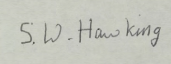
\includegraphics[width=0.35\linewidth]{figures/sw_sing.png}
\end{figure}
\begin{flushright}
S. W. Hawking
\end{flushright}

\begin{figure}[h]
    \hfill
    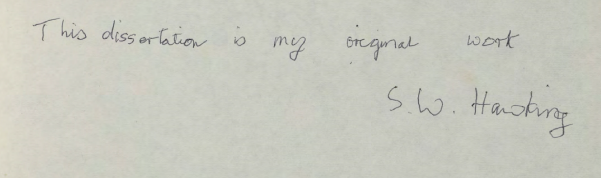
\includegraphics[width=1\linewidth]{figures/comment.png}
\end{figure}


\chapter{Chapter 1 \\The Hoyle--Narlikar Theory of Gravitation}

\sectiontoc{1. Introduction}

The success of Maxwell's equations has led to electrodynamics 
being normally formulated in terms of fields that have degrees 
of freedom independent of the particles in them. However, Gauss 
suggested that an action--at--a--distance theory in which the 
action travelled at a finite velocity might be possible. 
This idea was developed by Wheeler and Feynman~\cite{2,3} who derived 
their theory from an action principle that involved only direct 
interactions between pairs of particles. A feature of this theory 
was that the `pseudo'--fields introduced are the half--retarded 
plus half--advanced fields calculated from the world--lines of 
the particles. 

However, Wheeler and Feynman, and, in a different way, Hogarth~(3), 
were able to show that, provided certain cosmological conditions 
were satisfied, these fields could combine to give the observed field. 
Hoyle and Narlikar~\cite{4} extended the theory to general space--times 
and obtained similar theories for their `C'--field~\cite{5} and for the 
gravitational field~~\cite{6}. It is with these theories that this chapter 
is concerned.

It will be shown that in an expanding universe the advanced 
fields are infinite, and the retarded fields finite. 
This is because, unlike electric charges, all masses have the same sign.

\sectiontoc{The Boundary Condition}

Hoyle and Narlikar derive their theory from the action:
\[
A = \sum_{a \ne b} \sum \iint G(a,b)\, da\, db ,
\]
where the integration is over the world-lines of particles a, b...
In this expression G is a Green function
that satisfies the wave equation: 

\[
G(x,x')_{;ij}\, g^{ij} + \tfrac{1}{6} R\, G(x,x')
= \frac{\delta^{4}(x,x')}{\sqrt{-g}} \, .
\]


where \(S\) is the determinant of \(g_{ij}\).
Since the double sum in the action A is symmetrical between all pailrs of
particles a, b, only that part of G(a,b) that is symmetrical between a and b will contribute to the action
i.e. the action can be written

\[
A = \sum_{a \ne b} \sum \iint G^{*}(a,b)\, da\, db
\]

\noindent
where \quad 
\( G^{*}(a,b) = \tfrac{1}{2} G(a,b) + \tfrac{1}{2} G(b,a) \).

\medskip

Thus \quad \( G^{*} \) \quad must be the time-symmetric Green function, and can be written:

\[
G^{*} = \tfrac{1}{2} G_{\text{ret}} + \tfrac{1}{2} G_{\text{adv}}
\qquad \text{where } G_{\text{ret}}
\]
and \(G_{\text{adv}}\) are the retarded and advanced Green functions.
By requiring that the action be stationary under variations
of \(g_{ij}\), Hoyle and Narlikar obtain the field-equations:

\[
\Biggl[
\sum_{a \ne b} \sum \tfrac{1}{6} m^{(a)}(x)\, m^{(b)}(x)
\Biggr]
\left( R_{ik} - \tfrac{1}{2} g_{ik} R \right)
\]

\[
= - T_{ik}
+ \sum_{a \ne b} \sum \tfrac{1}{3} m^{(a)}
\Bigl[
g_{ik} m^{(b)r}{}_{;r}
- m^{(b)}_{;ik}
\Bigr]
+ 2 \bigl( m^{(a)}_{il}\, m^{(b)}_{j}{}^{l} \bigr)
- \tfrac{1}{4} g_{ik}\, m^{(a);r}\, m^{(b)}_{j;r}
\]
where \quad 
\( m^{(a)}(x) = \int G^{*}(x,a)\, da \).

\medskip

However, as a consequence of the particular choice of Green function, 
the contraction of the field--equations is satisfied identically. 
There are thus only 9 equations for the 10 components of \( g_{ij} \) 
and the system is indeterminate.

\medskip

Hoyle and Narlikar therefore impose 
\(\sum m^{(a)} = m_{0} = \text{const.}\), as the tenth equation. 
By then making the `smooth--fluid' approximation, that is by putting

\[
\sum_{a \ne b} \sum m^{(a)} m^{(b)} \approx m_{0}^{2},
\]

they obtain the Einstein field--equations:

\[
\tfrac{1}{6} m_{0}^{2}\left( R_{ik} - \tfrac{1}{2} R g_{ik} \right) 
= -T_{ik}.
\]

\medskip

There is an important difference, however, between these field--equations 
in the direct--particle interaction theory and in the usual general theory 
of relativity. In the general theory of relativity, any metric that satisfies the the field--equations is admissible, but in the direct--particle 
interaction theory only those solutions of the field--equations 
are admissible that satisfy the additional requirement:

\[
m_{0}(x) = \sum m^{(a)}(x) = \sum \int G^{*}(x,a)\, da
= \tfrac{1}{2} \sum \int G_{\text{ret}}(x,a)\, da 
+ \tfrac{1}{2} \sum \int G_{\text{adv}}(x,a)\, da
\]

\medskip

This requirement is highly restrictive; it will be shown that it 
is not satisfied for the cosmological solutions of the Einstein 
field--equations, and it appears that it cannot be satisfied for 
any models of the universe that either contain an infinite amount 
of matter or undergo infinite expansion.

\medskip

The difficulty is similar to that occurring in Newtonian theory 
when it is recognized that the universe might be infinite.  

The Newtonian potential \(\phi\) obeys the equation:

\[
\square \phi = - \kappa \rho \qquad (\rho > 0),
\]

where \(\rho\) is the density.
In an infinite static universe, \(\phi\) would be infinite, since 
the source always has the same sign. The difficulty was resolved 
when it was realized that the universe was expanding, since 
in an expanding universe the retarded solution of the above 
equation is finite by a sort of `red--shift' effect. The 
advanced solution will be infinite by a `blue--shift' effect. 
This is unimportant in Newtonian theory, since one is free 
to choose the solution of the equation and so may ignore the 
infinite advanced solution and take simply the finite 
retarded solution.

\medskip

Similarly in the direct--particle interaction theory the 
\(m\) field satisfies the equation:

\[
\square m - \tfrac{1}{6} R m = \mathcal{N} \qquad (\mathcal{N} > 0),
\]

where \(\mathcal{N}\) is the density of world--lines of particles. 
As in the Newtonian case, one may expect that the effect of the 
expansion of the universe will be to make the retarded solution 
finite and the advanced solution infinite. However, one is 
now not free to choose the finite retarded solution, for the 
equation is derived from a direct--particle interaction action--principle 
symmetric between pairs of particles, and one must choose for \(m\) 
half the sum of the retarded and advanced solutions. We would expect 
this to be infinite, and this is shown to be so in the next section.
\sectiontoc{The Cosmological Solutions}

The Robertson--Walker cosmological metrics have the form
\[
ds^{2} = dt^{2} - R^{2}(t) \left[ \frac{dr^{2}}{1 - \kappa r^{2}} 
+ r^{2}\bigl(d\theta^{2} + \sin^{2}\theta \, d\phi^{2}\bigr) \right].
\]

Since they are conformally flat, one can choose coordinates in which they become
\[
ds^{2} = \Omega^{2} \bigl[ d\tau^{2} - d\rho^{2} - \rho^{2}(d\theta^{2} + \sin^{2}\theta \, d\phi^{2}) \bigr]
= \Omega^{2} \eta_{ab}\, dx^{a} dx^{b},
\]
where \(\eta_{ab}\) is the flat--space metric tensor and
\[
\Omega = \Omega(\tau,\rho) = \frac{R(t)}{\sqrt{[t + \tfrac{1}{4}\kappa(\tau+\rho)^{2}][t + \tfrac{1}{4}\kappa(\tau-\rho)^{2}]}}. \tag{7}
\]

For example, for the Einstein--de Sitter universe
\[
\kappa = 0, \quad 
R(t) = \left(\tfrac{t}{T}\right)^{2/3}, 
\qquad (0 < t < \infty),
\]
\[
\Omega = R \cdot \left(\tfrac{\tau}{T}\right)^{2/3}, 
\qquad (0 < \tau < \infty),
\]
\[
\rho = \tau^{2/3}\, \xi^{1/3}.
\]

For the steady--state (de Sitter) universe
\[
\kappa = 0, \quad R(t) = e^{t/T}, 
\qquad (-\infty < t < \infty).
\]

\[
\Omega = R \cdot \frac{1}{\tau}, 
\qquad (-\infty < t < \infty),
\]
\[
r = \rho \left( \frac{\tau}{T} - T e^{t/T} \right).
\]

The Green function \( G^{*}(a,b) \) obeys the equation
\[
\square G^{*}(a,b) - \tfrac{1}{6} R\, G^{*}(a,b) 
= \frac{\delta^{4}(a,b)}{\sqrt{-g}}.
\]

From this it follows that
\[
\frac{1}{\Omega^{2}} \frac{\partial}{\partial x^{a}}
\left( \Omega^{2} \eta^{ab} \frac{\partial}{\partial x^{b}} G^{*} \right)
= \frac{1}{\Omega^{2}} \frac{\partial}{\partial x^{a}}
\left( \eta^{ab} \frac{\partial}{\partial x^{b}} S \right)
= \Omega^{-3}\, \delta^{4}(a,b).
\]

If we let \( G^{*} = \Omega^{-1} S \), then
\[
\Omega^{2} \frac{\partial}{\partial x^{a}}
\left( \eta^{ab} \frac{\partial}{\partial x^{b}} S \right)
= \delta^{4}(a,b).
\]

This is simply the flat--space Green function equation, and hence
\[
G^{*}(t_{1},0; t_{2},\rho) 
= \frac{\Omega(t_{1})}{8\pi \, \Omega(t_{2}) \, \rho}
\Bigl[ \delta(\rho - (t_{2}-t_{1})) + \delta(\rho + (t_{2}-t_{1})) \Bigr].
\]

The \(m\)--field is given by
\[
m(t,x) = \int G^{*} \mathcal{N}\, \sqrt{-g}\, dx
= \tfrac{1}{2}(m_{\text{ret}} + m_{\text{adv}}).
\]

For universes without creation (e.g.\ the Einstein--de Sitter universe),
\[
\mathcal{N} = R^{3} n, \qquad n = \text{const.}
\]

For Universes with creation (steady state) 
\(\mathcal{N} = n, \quad n = \text{const.}\)

\[
M_{\text{adv}}(\tau_{1}) = \Omega^{-1}(\tau_{1}) 
\int \frac{\mathcal{N}\,\Omega^{3}(\tau_{2})}{4\pi r}\, 4\pi r^{2}\, d\tau_{2},
\]

where the integration is over the future light cone. 
This will normally be infinite in an expanding universe, e.g.\ in the Einstein--de Sitter universe:

\[
M_{\text{adv}}(\tau_{1}) 
= \left(\frac{\tau_{1}}{T}\right)^{-2} 
\int_{\tau_{1}}^{\infty} n \left(\tfrac{\tau_{2}}{T}\right)^{2}\, d\tau_{2}
= \infty.
\]

In the steady--state universe
\[
M_{\text{adv}}(\tau_{1}) 
= \left(\tfrac{-T}{\tau_{1}}\right)^{-1} 
\int_{\tau_{1}}^{0} n \left(\tfrac{-T}{\tau_{2}}\right)^{3} (\tau_{2}-\tau_{1})\, d\tau_{2}
= \infty.
\]

\medskip

By contrast, on the other hand, we have
\[
M_{\text{ret}}(\tau_{1}) = \Omega^{-1}(\tau_{1}) 
\int \frac{\mathcal{N}\,\Omega^{3}}{4\pi r}\, 4\pi r^{2}\, dr,
\]

where the integration is over the past light cone. This will Normally be finite, e.g.\ in the Einstein--de Sitter universe
\[
M_{\text{ret}}(\tau_{1}) 
= \left(\frac{\tau_{1}}{T}\right)^{-2} 
\int_{0}^{\tau_{1}} n \left(\tfrac{\tau_{2}}{T}\right)^{2} (\tau_{2}-\tau_{1})\, d\tau_{2}
= \tfrac{1}{2} n T^{2}.
\]

While in the steady--state universe
\[
M_{\text{ret}}(\tau_{1}) 
= \left(\tfrac{-T}{\tau_{1}}\right)^{-1} 
\int_{-\infty}^{\tau_{1}} n \left(\tfrac{-T}{\tau_{2}}\right)^{3} (\tau_{2}-\tau_{1})\, d\tau_{2}
= \tfrac{1}{2} n T^{2}.
\]

Thus it can be seen that the solution \(m = \text{const.}\) of the equation
\[
\square m + \tfrac{1}{6} R m = \mathcal{N}
\]
is not, in a cosmological metric, the half--advanced plus half--retarded solution 
since this would be infinite. In fact, in the case of the Einstein--de Sitter 
and steady--state metrics, it is the pure retarded solution.

\sectiontoc{The `C'--Field}

Hoyle and Narlikar derive their direct--particle interaction theory of the 
`C'--field from the action
\[
A = \sum_{a \ne b} \iint \hat{G}(a,b)\, i_{a} \, k_{b}\, da^{4} db^{4}.
\]

where the suffixes \(a, b\) refer to differentiation of 
\(\hat{G}(a,b)\) on the world--lines of \(a, b\) respectively.  
\(\hat{G}\) is a Green function obeying the equation

\[
\square \hat{G}(x,x') = \frac{\delta^{4}(x,x')}{\sqrt{-g}}.
\]

We define the `C'--field by
\[
C(x) = \sum \hat{G}(x,a)\, i_{a}\, da^{i},
\]

and the matter--current \(J^{\kappa}\) by
\[
J^{\kappa}(y) = \sum \int \delta^{4}(y,b)\, db^{\kappa}.
\]

Then
\[
C(x) = \int \hat{G}(x,y)\, J^{\kappa}(y)_{;\kappa}\, \sqrt{-g}\, dx',
\]

so that
\[
\square C = J^{\kappa}{}_{;\kappa}.
\]

\medskip

We thus see that the sources of the `C'--field are the places 
where matter is created or destroyed.  

As in the case of the \(m\)--field, the Green function must be 
time--symmetric, that is
\[
\hat{G}(a,b) = \tfrac{1}{2}\, \hat{G}_{\text{ret}}(a,b) 
+ \tfrac{1}{2}\, \hat{G}_{\text{adv}}(a,b)
\]
Hoyle and Narlikar claim that if the action of the 
`C'--field is included along with the action of the `m'--field, 
a universe will be obtained that approximates to the steady--state 
universe on a large scale although there may be local irregularities. 
In this universe, the value of \(C\) will be finite and its gradient 
time--like and of unit magnitude.

\medskip

Given this universe, we may check it for consistency by calculating 
the advanced and retarded `C'--fields and finding if their sum is finite. 
We shall not do this directly but will show that the advanced field 
is infinite while the retarded field is finite.

\medskip

Consider a region in space--time bounded by a three--dimensional 
space--like hypersurface \(\mathcal{D}\) at the present time, 
and the past light cone \(\Sigma\) of some point \(P\) to the future of \(\mathcal{D}\).

By Gauss's theorem
\[
\int_{V} \square C \, \sqrt{-g}\, dx^{4} 
= \int_{\Sigma + \mathcal{D}} \frac{\partial C}{\partial n}\, dS
= \int J^{\kappa}{}_{;\kappa}\, \sqrt{-g}\, dx^{4}.
\]

Let the advanced field produced by sources within \(V\) be \(C'\).  
Then \(C'\) and \(\frac{\partial C'}{\partial n}\) will be zero on \(\Sigma\), and hence


\[
\int_{V} J^{\kappa}{}_{;\kappa} \, \sqrt{-g}\, dx^{4} 
= \int_{\mathcal{D}} \frac{\partial C'}{\partial n}\, dS.
\]

But \(J^{\kappa}{}_{;\kappa}\) is the rate of creation of matter \(= n\) (const.) 
in the steady--state universe, and hence
\[
\int_{\mathcal{D}} \frac{\partial C'}{\partial n}\, dS = nV.
\]

As the point \(P\) is taken further into the future, the volume 
of the region \(V\) tends to infinity. However, the area of the 
hypersurface \(\mathcal{D}\) tends to a finite limit owing to horizon 
effects. Therefore the gradient \(\tfrac{\partial C'}{\partial n}\) must be infinite.  
A similar calculation shows the gradient of the retarded 
field to be finite. Their sums cannot therefore give the 
field of unit gradient required by the Hoyle--Narlikar theory.

\medskip

It is worth noting that this result was obtained without 
assumptions of a smooth distribution of matter or of conformal flatness.
\sectiontoc{Conclusion}

It is one of the weaknesses of the Einstein theory of 
relativity that although it furnishes field equations it does 
not provide boundary conditions for them. Thus it does not 
give a unique model for the universe but allows a whole series 
of models. Clearly a theory that provided boundary conditions 
and thus restricted the possible solutions would be very 
attractive. The Hoyle--Narlikar theory does just that (the 
requirement that \( m = \tfrac{1}{2} m_{\text{ret}} + \tfrac{1}{2} m_{\text{adv}} \) 
is equivalent to a boundary condition). Unfortunately, as we 
have seen above, this condition excludes those models that 
seem to correspond to the actual universe, namely the 
Robertson--Walker models.

\medskip

The calculations given above have considered the universe 
as being filled with a uniform distribution of matter. This 
is legitimate if we are able to make the `smooth--fluid' 
approximation to obtain the Einstein equations. Alternatively, 
if this approximation is invalid, it cannot be said that the 
theory yields the Einstein equations.

\medskip

It might possibly be that local irregularities could make 
\(m_{\text{adv}}\) finite, but this has certainly not been demonstrated 
and seems unlikely in view of the fact that, in the Hoyle--Narlikar 
direct--particle interaction theory of their `C'--field,

which is derived from a very similar action--principle, it can 
be shown without assuming a smooth distribution that the 
advanced `C' field will be infinite in an expanding universe 
with creation.

\medskip

The reason that it is possible to formulate a direct--particle 
interaction theory of electrodynamics that does not encounter 
this difficulty of having the advanced solution infinite is 
that in electrodynamics there are equal numbers of sources 
of positive and negative sign. Their fields can cancel each 
other out and the total field can be zero apart from local 
irregularities. This suggests that a possible way to save the 
Hoyle--Narlikar theory would be to allow masses of both positive 
and negative sign. The action would be
\[
A = \sum_{a \ne b} q_{a} q_{b} \iint G^{*}(a,b)\, da\, db, 
\qquad (q_{a}, q_{b} = \pm 1),
\]
where \(q_{a}, q_{b}\) are gravitational charges analogous to 
electric charges. Particles of positive \(q\) in a positive 
`m'--field and particles of negative \(q\) in a negative 
`m'--field would have the normal gravitational properties, 
that is, they would have positive gravitational and inertial masses.

A particle of negative \(q\) in a positive `m'--field would 
still follow a geodesic. Therefore it would be attracted by 
a particle of positive \(q\). Its own gravitational effect 
however would be to repel all other particles. Thus it would 
have the properties of the negative mass described by Bondi~(8), 
that is, negative gravitational mass and negative inertial mass.

\medskip

Since there does not seem to be any matter having these 
properties in our region of space (where \(m = \text{const.} > 0\)) 
there must clearly be separation on a very large scale. It 
would not be possible to identify particles of negative \(q\) 
with antimatter, since it is known that antimatter has positive 
inertial mass. However, the introduction of negative masses 
would probably raise more difficulties than it would solve.






\sectiontoc{References}

\begin{enumerate}
\item J. A. Wheeler and R. P. Feynman, 
\textit{Rev. Mod. Phys.} \textbf{17}, 157 (1945).

\item J. A. Wheeler and R. P. Feynman, 
\textit{Rev. Mod. Phys.} \textbf{21}, 425 (1949).

\item J. E. Hogarth, 
\textit{Proc. Roy. Soc. A} \textbf{267}, 365 (1962).

\item F. Hoyle and J. V. Narlikar, 
\textit{Proc. Roy. Soc. A} \textbf{277}, 1 (1964a).

\item F. Hoyle and J. V. Narlikar, 
\textit{Proc. Roy. Soc. A} \textbf{282}, 178 (1964b).

\item F. Hoyle and J. V. Narlikar, 
\textit{Proc. Roy. Soc. A} \textbf{282}, 191 (1964c).

\item L. Infeld and A. Schild, 
\textit{Phys. Rev.} \textbf{68}, 250 (1945).

\item H. Bondi, 
\textit{Rev. Mod. Phys.} \textbf{29}, 423 (1957).
\end{enumerate}




\chapter{Chapter 2 \\Perturbations}
\sectiontoc{Introduction}

Perturbations of a spatially isotropic and homogeneous expanding 
universe have been investigated in a Newtonian approximation by 
Bonnor~\cite{Bonnor1957} and relativistically by Lifshitz~\cite{Lifshitz1946}, 
Lifshitz and Khalatnikov~\cite{LifshitzKhalatnikov1963}, 
and Irvine~\cite{Irvine1965}. Their method was to consider small 
variations of the metric tensor. This has the disadvantage that the 
metric tensor is not a physically significant quantity, since one 
cannot directly measure it, but only its second derivatives. 
It is thus not obvious what the physical interpretation of a given 
perturbation of the metric is. Indeed it need have no physical 
significance at all, but merely correspond to a coordinate transformation. 
Instead it seems preferable to deal in terms of perturbations of the 
physically significant quantity, the curvature.
\sectiontoc{Notation}

Space--time is represented as a four--dimensional Riemannian space 
with metric tensor \(g_{ab}\) of signature \(+2\). Covariant differentiation 
in this space is indicated by a semi--colon. Square brackets around 
indices indicate antisymmetrisation and round brackets symmetrisation.  
The conventions for the Riemann and Ricci tensors are:
\[
\nabla_{a;[bc]} = 2\, R^{p}{}_{a c b}\, \nabla_{p},
\]
\[
R_{ab} = R^{p}{}_{a p b}.
\]

\(\eta_{abcd}\) is the alternating tensor.  

Units are such that \(\kappa\), the gravitational constant, and \(c\), the speed of light, are one


\sectiontoc{The Field Equations}

We assume the Einstein equations:
\[
R_{ab} - \tfrac{1}{2} g_{ab} R = -T_{ab}
\]
where \(T_{ab}\) is the energy--momentum tensor of matter.  
We will assume that the matter consists of a perfect fluid. Then,
\[
T_{ab} = \mu\, u_{a} u_{b} + p\, h_{ab}
\]
where \(u_{a}\) is the velocity of the fluid, \(u_{a} u^{a} = -1\) :
\[
\mu \ \text{is the density}, \qquad 
p \ \text{is the pressure},
\]
\[
h_{ab} = g_{ab} + u_{a} u_{b} \quad 
\text{is the projection operator into the hyperplane orthogonal to } u_{a},
\]
\[
h_{ab} u^{b} = 0.
\]

\medskip

We decompose the gradient of the velocity vector \(u_{a}\) as
\[
u_{a;b} = \omega_{ab} + \sigma_{ab} + \tfrac{1}{3} h_{ab} \, \theta - \dot{u}_{a} u_{b}
\]
where
\[
\dot{u}_{a} = u_{a;b} u^{b} \quad \text{is the acceleration},
\]
\[
\theta = u^{a}{}_{;a} \quad \text{is the expansion},
\]
\[
\sigma_{ab} = u_{(c;d)} h^{c}{}_{a} h^{d}{}_{b} - \tfrac{1}{3} h_{ab} \theta 
\quad \text{is the shear},
\]
\[
\omega_{ab} = u_{[c;d]} h^{c}{}_{a} h^{d}{}_{b} 
\quad \text{is the rotation of the flow lines } u^{a}.
\]

We define the rotation vector \(\omega_{a}\) as
\[
\omega_{a} = \tfrac{1}{2} \eta_{abcd} \, \omega^{cd} u^{b}.
\]

\medskip

We may decompose the Riemann tensor \(R_{abcd}\) into the Ricci tensor 
\(R_{ab}\) and the Weyl tensor \(C_{abcd}\):
\[
R_{abcd} = C_{abcd} - g_{a[c} R_{d]b} + g_{b[c} R_{d]a} - \tfrac{1}{3} R g_{a[c} g_{d]b},
\]
\[
C_{abcd} = C_{[ab][cd]}, \qquad C^{a}{}_{bca} = 0 = C_{a[ bcd ]}.
\]

\(C_{abcd}\) is that part of the curvature that is not determined locally by 
the matter. It may thus be taken as representing the free gravitational 
field (Jordan, Ehlers and Kundt\cite{JordanKundt1960}).  
We may decompose it into its ``electric'' and ``magnetic'' components:
\[
E_{ab} = - C_{a b p q}\, u^{p} u^{q}, 
\]
\[
H_{ab} = - \tfrac{1}{2} C_{a p q r}\, \eta^{qr}{}_{bs}\, u^{p} u^{s},
\]
\[
C_{ab}{}^{cd} 
= 8 u_{[a} E_{b]}{}^{[c} u^{d]} 
+ 4 \delta_{[a}{}^{[c} E_{b]}{}^{d]}
- 2 \eta_{ab}{}^{cd} u^{p} H_{p}{}^{[c} u^{d]}
- 2 \eta^{cdrs} u_{r} H_{s[a} u_{b]} .
\]

\[
E_{ab} = E_{(ab)}, 
\qquad H_{ab} = H_{(ab)},
\]
\[
E_{a}{}^{a} = H_{a}{}^{a} = 0,
\]
\[
E_{ab} u^{b} = H_{ab} u^{b} = 0.
\]

\(E_{ab}\) and \(H_{ab}\) each have five independent components.  

We regard the Bianchi identities,
\[
R_{ab[cd;e]} = 0,
\]
as field equations for the free gravitational field.  

Then
\[
C_{abc d}{}^{d} = - R_{c[b;a]} + \tfrac{1}{6} g_{c[b} R_{;a]},
\]
(Kundt and Trümper\cite{KundtTrumper1962}).

Using the decompositions given above, we may write these in a form 
analogous to the Maxwell equations:
\begin{align}
h^{b}{}_{e} H_{bc;d} h^{cf} + 3 H_{ab} \omega^{b} - \eta_{abcd} u^{b} \sigma^{c}{}_{e} H^{de} 
&= \tfrac{3}{2} h_{a}{}^{b} \mu_{;b}, \tag{1} \\[1ex]
h^{b}{}_{e} E_{bc;d} h^{cf} + 3 E_{ab} \omega^{b} - \eta_{abcd} u^{b} \sigma^{c}{}_{e} E^{de} 
&= (\mu + p) \, \omega_{a}, \tag{2} \\[1ex]
\perp \dot{E}_{ab} + h^{c}{}_{(a} \eta_{b)cde} u^{c} H^{de} + E_{ab} \theta - E^{c}{}_{(a} \omega_{b)c} 
&- E^{c}{}_{(a} \sigma_{b)c} - \eta_{cde(a} \eta_{bpqr} u^{c} u^{p} \sigma^{d}{}_{q} E^{er} \notag \\ 
&+ 2 H^{c}{}_{(a} \eta_{b)cde} u^{c} \dot{u}^{e} = -\tfrac{1}{2} (\mu + p) \sigma_{ab}, \tag{3} \\[1ex]
\perp \dot{H}_{ab} - h^{c}{}_{(a} \eta_{b)cde} u^{c} E^{de} + H_{ab} \theta - H^{c}{}_{(a} \omega_{b)c} 
&- H^{c}{}_{(a} \sigma_{b)c} - \eta_{cde(a} \eta_{bpqr} u^{c} u^{p} \sigma^{d}{}_{q} H^{er} \notag \\ 
&+ 2 H^{c}{}_{(a} \eta_{b)cde} u^{c} \dot{u}^{e} = 0. \tag{4}
\end{align}

where \(\perp\) indicates projection by \(h_{ab}\) orthogonal to \(u_{a}\) (c.f.\ Trümper (7)).  

\medskip

The contracted Bianchi identities give,
\begin{align}
(R_{ab} - \tfrac{1}{2} g_{ab} R)^{;b} &= - T_{ab}{}^{;b} = 0, \notag \\
\dot{\mu} + (\mu + p) \theta &= 0, \tag{5} \\
(\mu + p) \dot{u}_{a} + p_{,b} h^{b}{}_{a} &= 0. \tag{6}
\end{align}

The definition of the Riemann tensor is,
\[
u_{a;[bc]} = 2 R_{a p b c} u^{p}.
\]

Using the decompositions as above we may obtain what may be regarded 
as ``equations of motion''.

\begin{align}
\dot{\theta} &= 2 \omega^{2} - 2 \sigma^{2} - \tfrac{1}{3} \theta^{2} + \dot{u}^{a}{}_{;a} 
- \tfrac{1}{2} (\mu + 3p), \tag{7} \\[1ex]
\perp \dot{\omega}_{ab} &= - \tfrac{2}{3} \omega_{ab} \theta 
+ 2 \sigma_{c[a} \omega_{b]}{}^{c} 
+ \dot{u}_{[p;q]} h^{p}{}_{a} h^{q}{}_{b}, \tag{8} \\[1ex]
\perp \dot{\sigma}_{ab} &= E_{ab} - \omega_{ac} \omega^{c}{}_{b} - \sigma_{ac} \sigma^{c}{}_{b} 
- \tfrac{2}{3} \sigma_{ab} \theta \notag \\
&\quad - \tfrac{1}{3} h_{ab} (2 \omega^{2} - 2 \sigma^{2} + \dot{u}^{c}{}_{;c}) 
+ \dot{u}_{a} \dot{u}_{b} 
+ \dot{u}_{(p;q)} h^{p}{}_{a} h^{q}{}_{b}, \tag{9}
\end{align}

where \(\; 2\omega^{2} = \omega_{ab} \omega^{ab}, \quad 2\sigma^{2} = \sigma_{ab} \sigma^{ab}\).

\medskip

We also obtain what may be regarded as equations of constraint:
\begin{align}
\theta_{,b} h^{ba} &= \tfrac{3}{2} \Big[ 
  (\omega_{bc;b} + \sigma^{c}{}_{b;c}) h^{ca} 
  - \dot{u}^{b} (\omega_{ab} + \sigma_{ab}) \Big], \tag{10} \\[1ex]
\omega^{a}{}_{;a} &= 2 \omega_{a} \dot{u}^{a}, \tag{11} \\[1ex]
H_{ab} &= - h^{c}{}_{(a} \eta_{b)cde} u^{c} 
\left( \omega^{d;e} + \sigma^{d;e} \right). \tag{12}
\end{align}

\medskip

We consider perturbations of a universe that in the undisturbed state 
is conformally flat, that is
\[
C_{abcd} = 0.
\]

By equations (1)–(3), this implies
\[
\sigma_{ab} = \omega_{ab} = 0, 
\qquad h^{b}{}_{a} \mu_{;b} = 0, 
\qquad \theta_{;b} h^{ba}.
\]
If we assume an equation of state of the form, $\mu = \mu(\rho)$,  
then by (6), (10),
\[
\mu_{,b} h^{b}{}_{a} = 0 = \dot{\mu} u_{a}.
\]

This implies that the universe is spatially homogeneous and isotropic 
since there is no direction defined in the 3-space orthogonal to $u_{a}$.

In this universe we consider small perturbations of the motion 
of the fluid and of the Weyl tensor. We neglect products of small 
quantities and perform derivatives with respect to the undisturbed 
metric. Since all the quantities we are interested in with the 
exception of the scalars, $\mu, \dot{\mu}, \theta$ have unperturbed value zero, we 
avoid perturbations that merely represent coordinate transformation 
and have no physical significance.

To the first order the equations (1)–(4) and (7)–(9) are
\begin{align}
E_{ab}{}^{;b} &= \tfrac{1}{3} h_{a}{}^{b} \mu_{,b}, \tag{13}\\
H_{ab}{}^{;b} &= (\mu + h)\, \omega_{a}, \tag{14}\\
\dot{E}_{ab} + E_{c(a}\theta + h^{c}{}_{(a}\eta_{b)de}u^{d}H^{e}{}_{c}{}^{;c} 
  &= -\tfrac{1}{2}(\mu + h)\,\sigma_{ab}, \tag{15}\\
\dot{H}_{ab} + H_{c(a}\theta - h^{c}{}_{(a}\eta_{b)de}u^{d}E^{e}{}_{c}{}^{;c} &= 0, \tag{16}\\
\dot{\theta} &= -\tfrac{1}{3}\theta^{2} + \dot{u}^{a}{}_{;a} - \tfrac{1}{2}(\mu + 3h), \tag{17}\\
\dot{\omega}_{ab} &= -\tfrac{2}{3}\omega_{ab}\theta + \dot{u}_{[a;p]} h^{p}{}_{b} h^{q}{}_{a}, \tag{18}\\
\dot{\sigma}_{ab} &= E_{ab} - \tfrac{2}{3}\sigma_{ab}\theta - \tfrac{1}{3}h_{ab}\dot{u}^{c}{}_{;c}
   + \dot{u}_{(p;q)} h^{p}{}_{a} h^{q}{}_{b}. \tag{19}
\end{align}
From these we see that perturbations of rotation or of $E_{ab}$ or $H_{ab}$ do 
not produce perturbations of the expansion or the density. Nor do 
perturbations of $E_{ab}$ and $H_{ab}$ produce rotational perturbations.  

\sectiontoc{The Undisturbed Metric}

Since in the unperturbed state the rotation and acceleration 
are zero, $u_{a}$ must be hypersurface orthogonal.

\[
u_{a} = \tau_{,a},
\]

where $\tau$ measures the proper time along the world lines. As the 
surfaces $\tau = \text{constant}$ are homogeneous and isotropic they must be 
3-surfaces of constant curvature. Therefore the metric can be 
written,

\[
ds^{2} = - d\tau^{2} + \Omega^{2} d\gamma^{2},
\]

where  

\[
\Omega = \Omega(\tau),
\]

\[
d\gamma^{2} \quad \text{is the line element of a space of zero or unit positive or negative curvature.}
\]

We define $t$ by  

\[
\frac{dt}{d\tau} = \frac{1}{\Omega},
\]

then  

\[
ds^{2} = \Omega^{2} \left( -dt^{2} + d\gamma^{2} \right).
\]

In this metric,  

\[
u_{a} = (-\Omega, 0, 0, 0),
\]

\[
\therefore \quad \theta = \frac{3 \dot{\Omega}}{\Omega} = \frac{3 \Omega'}{\Omega^{2}}
\]

\[
\text{(prime denotes differentiation with respect to $t$).}
\]
Then, by (5), (7)
\begin{align}
\dot{\mu} &= -(\mu + h)\,\frac{3\dot{\Omega}}{\Omega}, \tag{20}\\[6pt]
3\frac{\ddot{\Omega}}{\Omega} &= -\tfrac{1}{2}(\mu + 3h). \tag{21}
\end{align}

If we know the relation between $\mu$ and $h$, we may determine $\Omega$.  
We will consider the two extreme cases, $h=0$ (dust) and $h=\tfrac{1}{3}\mu$ (radiation).  
Any physical situation should lie between these.

\subsubsection*{For $h = 0$}

By (20), \quad $\mu = \dfrac{M}{\Omega^{3}}$, \quad $M = \text{const}.$

\[
\therefore \quad \frac{3}{M}\,\Omega \ddot{\Omega} - \tfrac{1}{2}\Omega^{2} = 0,
\]

\[
\therefore \quad \frac{3}{M}\,\dot{\Omega}^{2} - \frac{1}{\Omega} = E, 
\qquad E = \text{const}.
\]

\paragraph{(a) For $E>0$,}
\[
\Omega = \tfrac{1}{2E}\Big(\cosh \sqrt{\tfrac{E M}{3}}\,t - 1\Big), 
\qquad 
\tau = \tfrac{1}{2E}\Big(\sqrt{\tfrac{3}{E M}}\,\sinh \sqrt{\tfrac{E M}{3}}\,t + t \Big);
\]

\paragraph{(b) For $E=0$,}
\[
\Omega = \frac{M}{12}\,t^{2}, 
\qquad 
\tau = \frac{M}{36}\,t^{3};
\]

\paragraph{(c) For $E<0$,}
\[
\Omega = -\tfrac{1}{2E}\Big(1 - \cos \sqrt{-\tfrac{E M}{3}}\,t \Big), 
\qquad 
\tau = -\tfrac{1}{2E}\Big(t - \sqrt{\tfrac{3}{-E M}} \sin \sqrt{-\tfrac{E M}{3}}\,t \Big).
\]

\medskip
$E$ represents the energy (kinetic + potential) per unit mass.  
If it is non–negative the universe will expand indefinitely, otherwise it will eventually contract again.
By the Gauss–Codazzi equations $^{*}R$, the curvature of the 
hypersurface $\tau = \text{const.}$ is  

\[
^{*}R = 2\left(-\tfrac{1}{3}\theta^{2} + \mu\right)
      = -\frac{2 E M}{\Omega^{2}}.
\]

If $E > 0$, \quad $^{*}R = -\dfrac{6}{\Omega^{2}}, \qquad M = \dfrac{3}{E}$;

\[
E = 0, \quad {}^{*}R = 0;
\]

If \(E < 0\), \quad
\({}^{*}R = \dfrac{6}{\Omega^{2}}, \qquad M = -\dfrac{3}{E}\).


\subsubsection*{For $h = \tfrac{1}{3}\mu$}

\[
\dot{\mu} = -4\frac{\dot{\Omega}}{\Omega},
\]

\[
3\frac{\ddot{\Omega}}{\Omega} = -\mu, 
\qquad \mu = \frac{M}{\Omega^{4}},
\]

\[
\therefore \quad \frac{3}{M}\dot{\Omega}^{2} - \frac{1}{\Omega^{2}} = E.
\]

\paragraph{(a) For $E > 0$:}
\[
\Omega = \frac{1}{E}\sinh t, 
\qquad \tau = \frac{1}{E}(\cosh t - 1), 
\qquad {}^{*}R = -\frac{6}{\Omega^{2}};
\]

\paragraph{(b) For $E = 0$:}
\[
\Omega = t, 
\qquad \tau = \tfrac{1}{2}t^{2}, 
\qquad {}^{*}R = 0;
\]

\paragraph{(c) For $E < 0$:}
\[
\Omega = \frac{1}{E}\sin t, 
\qquad \tau = \frac{1}{E}(\cos t - 1), 
\qquad {}^{*}R = \frac{6}{\Omega^{2}}.
\]

\sectiontoc{Rotational Perturbations}

By (6)
\[
\dot{u}_{[c;d]} h^{c}{}_{a} h^{d}{}_{b} 
   = -\frac{\omega_{ab}\,\dot{h}}{\mu + h}.
\]
\[
\dot{\omega}_{ab} = -\omega_{ab}\left(\tfrac{2}{3}\theta + \tfrac{\dot{h}}{\mu + h}\right).
\]

For $h = 0$,
\[
\omega = \frac{\omega_{0}}{\Omega^{2}}.
\]

For $h = \tfrac{\mu}{3}$,
\[
\dot{\omega} = -\omega\left(\tfrac{2}{3}\theta + \tfrac{1}{4}\frac{\dot{\mu}}{\mu}\right)
= -\tfrac{5}{3}\omega\theta,
\]
\[
\therefore \quad \omega = \frac{\omega_{0}}{\Omega^{5}}.
\]

Thus rotation dies away as the universe expands.  
This is in fact a statement of the conservation of angular momentum in an expanding universe.

\sectiontoc{Perturbations of Density}

For $h = 0$ we have the equations,
\[
\dot{\mu} = -\mu\theta,
\]
\[
\dot{\theta} = -\tfrac{1}{3}\theta^{2} - \tfrac{1}{2}\mu.
\]

These involve no spatial derivatives. Thus the behaviour of one 
region is unaffected by the behaviour of another. Perturbations 
will consist in some regions having slightly higher or lower values 
of $\theta$ than the average. If the universe as whole has a value of $E$ 
greater than zero, a small perturbation will still have $E$ greater 
than zero and will continue to expand. It will not contract to form a galaxy. If the universe has a value of $E$ less than zero, a 
small perturbation can contract. However it will only begin 
contracting at a time $\delta\tau$ earlier than the whole universe begins 
contracting, where  

\[
\frac{\delta\tau}{\tau_{c}} = \frac{\delta E}{E_{0}},
\]

$\tau_{c}$ is the time at which the whole universe begins contracting.  
There is only any real instability when $E=0$. This case is of 
measure zero relative to all the possible values $E$ can have.  
However this cannot really be used as an argument to dismiss it 
as there might be some reason why the universe should have $E=0$.

For a region with energy $- \delta E$, in a universe with $E=0$,

\[
\Omega = \frac{1}{4\delta E}\left(t^{2} - \frac{t^{4}}{12} + \cdots \right),
\]

\[
\tau = \frac{1}{12\delta E}\left(t^{3} - \frac{t^{5}}{20} + \cdots \right),
\]

\[
\mu = \frac{3}{6E\,\Omega^{2}} = \frac{4}{3}\tau^{-2}
     \left(1 + \frac{(\delta E)^{2/3}}{2^{1/3}}\,\tau^{2/3} + \cdots \right).
\]

For $E=0$, \quad $\mu = \tfrac{4}{3}\tau^{-2}$.

Thus the perturbation grows only as $\tau^{2/3}$.  
This is not fast enough to produce galaxies from statistical fluctuations 
even if these could occur. However, since an evolutionary universe has 
a particle horizon (Rindler\,(8), Penrose\,(9)) different parts do not 
communicate in the early stages. This makes it even more difficult for 
statistical fluctuations to occur over a region until light had time 
to cross the region.

\subsubsection*{For $h = \tfrac{\mu}{3}$}

\[
\dot{\mu} = -\tfrac{4}{3}\mu\theta,
\]
\[
\dot{\theta} = -\tfrac{1}{3}\theta^{2} - \mu + \dot{u}^{a}{}_{;a},
\]
\[
\dot{u}_{a} = -\frac{h^{b}{}_{a}\,\mu_{,b}}{4\mu}.
\]

As before, a perturbation cannot contract unless it has a negative 
value of $E$. The action of the pressure forces makes it still more 
difficult for it to contract. Eliminating $\theta$,

\[
\mu \ddot{\mu} - \tfrac{5}{4}\dot{\mu}^{2} - \tfrac{5}{3}\mu^{3} + \tfrac{4}{3}\mu^{2}\dot{u}^{a}{}_{;a} = 0,
\]

\[
\ddot{u}^{a} = \dot{u}^{a}{}_{;b}\,h^{b}{}_{a}{}^{b} + \dot{u}^{a}\dot{u}^{a}
= -\tfrac{1}{4}\,h^{ac}\frac{(h^{b}{}_{a}\mu_{,b})_{;c}}{\mu}
\quad \text{to our approximation.}
\]

\[
h^{ac}\nabla_{c} h^{b}{}_{a}\nabla_{b}
\]
is the Laplacian in the hypersurface $\tau = \text{constant}$.  

We represent the perturbation as a sum of eigenfunctions $S^{(n)}$ of 
this operator, where  

\[
S^{(n)}{}_{;a}u^{a} = 0,
\]

\[
h^{ac}(h^{b}{}_{a}S^{(n)}{}_{,b})_{;c} 
= -\frac{n^{2}}{\Omega^{2}}\,S^{(n)}.
\]

These eigenfunctions will be hyperspherical and pseudohyperspherical 
harmonics in cases (c) and (a) respectively and plane waves in case (b).  
In case (c) $n$ will take only discrete values but in (a) and (b) it will take all positive values.

\[
\mu = \mu_{0}\left(1 + \sum_{n} B^{(n)} S^{(n)}\right),
\]

where $\mu_{0}$ is the undisturbed density.

\[
\ddot{B}^{(n)}\mu_{0} - \tfrac{1}{2}\dot{B}^{(n)}\mu_{0} - B^{(n)}\left(\tfrac{4}{3}\mu_{0}^{2} - \tfrac{n^{2}}{3\Omega^{2}}\mu_{0}\right) = 0.
\]

As long as $\mu_{0} > \tfrac{n^{2}}{4\Omega^{2}}$, $B^{(n)}$ will grow.  

For $\mu_{0} \gg \tfrac{n^{2}}{4\Omega^{2}}$,

\[
B^{(n)} \simeq C\,\tau + D\,\tau^{-1}.
\]

These perturbations grow for as long as light has not had time to 
travel a significant distance compared to the scale of the perturbation 
($\sim \tfrac{\Omega}{n}$). Until that time pressure forces cannot act to even out 
perturbations.

When $\tfrac{n^{2}}{\Omega^{2}} \gg \mu_{0}$,

\[
\ddot{B}^{(n)} + \dot{B}^{(n)}\frac{\dot{\Omega}}{\Omega} + \tfrac{n^{2}}{3}B^{(n)} = 0,
\]

\[
\therefore \quad B^{(n)} \simeq C\,\Omega^{-\tfrac{1}{2}} e^{\pm i \tfrac{n}{\sqrt{3}} t}.
\]

We obtain sound waves whose amplitude decreases with time.  
These results confirm those obtained by Lifshitz and Khalatnikov\,(3).

From the foregoing we see that galaxies cannot form as the result 
of the growth of small perturbations. We may expect that other non–
gravitational forces will have an effect smaller than pressure equal 
\sectiontoc{The Steady-state Universe}

To obtain the steady-state universe we must add extra terms to 
the energy–momentum tensor. Hoyle and Narlikar\,(10) use,

\[
T_{ab} = \mu\, u_{a} u_{b} + h_{ab} - C_{a} C_{b} 
+ \tfrac{1}{2} g_{ab} C_{c} C^{d}. \tag{20}
\]

where,  

\[
C_{a} = C_{;a}, \qquad 
C_{;a}{}^{a} = -\dot{j}_{a}{}^{a}, \qquad 
j_{a} = -(\mu + h) u_{a}.
\]

Since $T_{ab}{}^{;b} = 0$,

\[
\dot{\mu} + (\mu + h)\theta + u^{a} C_{\mu} C_{b}{}^{;b} = 0, \tag{21}
\]

\[
(\mu + h)\dot{u}_{a} + h^{b}{}_{a} h^{c}{}_{b} 
- h^{b}{}_{a} C_{b} C_{d}{}^{;d} = 0. \tag{22}
\]

There is a difficulty here, if we require that the ``$C$'' field


should not produce acceleration or, in other words, that the matter 
created should have the same velocity as the matter already in 
existence. We must then have

\[
h^{b}{}_{a} C_{b} = 0. \tag{23}
\]

However since $C$ is a scalar, this implies that the rotation of the 
medium is zero. On the other hand if (23) does not hold, the equations 
are indeterminate (c.f. Raychaudhuri and Bannerjee\,(11)). In order to 
have a determinate set of equations we will adopt (23) but drop the 
requirement that $C_{a}$ is the gradient of a scalar. The condition (23) 
is not very satisfactory but it is difficult to think of one more 
satisfactory. Hoyle and Narlikar\,(12) seek to avoid this difficulty 
by taking a particle rather than a fluid picture. However this has a 
serious drawback since it leads to infinite fields (Hawking\,(13)).

From (17),

\[
C_{a} = -u_{a}\left[1 - \frac{\dot{\mu}}{\mu + \dot{\mu} + (\mu + h)\theta}\right].
\]

\[
\therefore \quad C^{a}{}_{;a} = -(\dot{\mu}+h) - (\mu+h)\theta,
\]

\[
= -\theta\left(1 - \frac{\dot{\mu}}{\mu + \dot{\mu} + (\mu + h)\theta}\right)
+ \frac{\dot{\mu}}{\mu + \dot{\mu} + (\mu + h)\theta}.
\]


For $\mu \gg h$
\[
(\dot{\mu} + \dot{h}) = \theta \big(1 - (\mu + h)\big),
\]
\[
\therefore \quad (\mu + h) \to 1.
\]

Thus, small perturbations of density die away. Moreover equation (18) 
still holds, and therefore rotational perturbations also die away.  
Equation (19) now becomes

\[
\dot{\theta} = -\tfrac{1}{3}\theta^{2} - \tfrac{1}{2}(\mu + 3h) + 1,
\]
\[
\therefore \quad \theta \to \sqrt{3\left(\tfrac{1}{2} - h\right)}.
\]

These results confirm those obtained by Hoyle and Narlikar\,(14). We 
see therefore that galaxies cannot be formed in the steady-state 
universe by the growth of small perturbations. However this does not 
exclude the possibility that there might be a self-perpetuating 
system of finite perturbations which could produce galaxies.  
(Sciama\,(15), Roxburgh and Saffman\,(16)).

\sectiontoc{Gravitational Waves}

We now consider perturbations of the Weyl tensor that do not 
arise from rotational or density perturbations, that is,
\[
E_{ab}{}^{;b} = H_{ab}{}^{;b} = 0
\]

Multiplying (15) by $u^{c}\nabla_{c}$, and (16) by 
$h^{a}{}_{(c}\eta_{b)}{}^{rs}u_{r}\nabla_{s}$, 
we obtain, after a lot of reduction,
\[
\ddot{E}_{ab} - \left( E_{cd;e}\, h^{c}{}_{f} h^{d}{}_{g} h^{e}{}_{(a}\, h^{fg}{}_{b)} \right)
+ h^{kl} h_{a}{}^{t} h_{b}{}^{s}\, \tfrac{7}{3}\,\dot{E}_{ab}\,\theta
\]
\[
+ E_{ab}\left(\dot{\theta} + \tfrac{4}{3}\theta^{2} + \tfrac{1}{3}(\mu + 3h)\right) 
+ \sigma_{ab}\left(\tfrac{1}{3}\theta(\mu+h) + \tfrac{1}{2}(\dot{\mu}+\dot{h})\right) = 0. \tag{24}
\]

In empty space with a non-expanding congruence $u^{a}$ this reduces to 
the usual form of the linearised theory,
\[
\square^{*} E_{ab} = 0.
\]

The second term in (24) is the Laplacian in the hypersurface 
$\tau = \text{constant}$, acting on $E_{ab}$. We will write $E_{ab}$ as a sum of 
eigenfunctions of this operator,
\[
E_{ab} = \sum A^{(n)} V_{ab}^{(n)},
\]
where
\[
\dot{V}_{ab}^{(n)} = 0, \qquad
\left( V_{cd;e}\, h^{c}{}_{f} h^{d}{}_{g} h^{e}{}_{(a} h^{fg}{}_{b)} \right)
= -\frac{n^{2}}{\Omega^{2}}\, V_{ab}^{(n)},
\]
\[
V_{ab}{}^{;b} = 0, \qquad V_{a}{}^{a} = 0.
\]

Then
\[
\dot{E}_{ab} = \sum \frac{A^{(n)}}{\Omega}\, V_{ab}^{(n)},
\qquad
\ddot{E}_{ab} = \sum \left[\frac{\dot{A}^{(n)}}{\Omega^{2}} 
- \frac{A^{(n)}}{\Omega^{2}}\right] V_{ab}^{(n)}.
\]

Similarly,
\[
\sigma_{ab} = \sum D^{(n)} V_{ab}^{(n)}.
\]

Then by (19)
\[
D'^{(n)} = \Omega A^{(n)} - 2D^{(n)}\frac{\Omega'}{\Omega}.
\]

Substituting in (24),
\[
A''^{(n)} + \frac{6\Omega'}{\Omega} A'^{(n)} + A^{(n)} 
\left[ n^{2} + 3\frac{\Omega''}{\Omega} + 6\frac{\Omega'^{2}}{\Omega^{2}} 
+ \tfrac{1}{3}(\mu + 3h)\Omega^{2}\right]
+ D^{(n)}\left[\Omega(\mu+h) + \tfrac{1}{2}\Omega^{2}(\dot{\mu}+\dot{h})\right] = 0.
\]

We may differentiate again and substitute for $D'$.  
For $n \gg 1$ and $\Omega \gg \tfrac{n^{2}}{h^{2}}$,
\[
A^{(n)} \simeq \frac{1}{\Omega^{3/2}} e^{i n t}.
\]

So the gravitational field $E_{ab}$ decreases as $\Omega^{-1}$ and the 
``energy'' $\tfrac{1}{2}(E_{ab}E^{ab} + H_{ab}H^{ab})$ as $\Omega^{-6}$.  
We might expect this as the Bianchi identities may be written, to the 
linear approximation,
\[
\Omega\, g^{ed} \frac{\partial}{\partial x^{e}}
\left(\Omega^{2} C_{abcd}\right) = J_{abc}.
\]

Therefore if the interaction with the matter could be neglected 
$C_{abcd}$ would be proportional to $\Omega$ and $E_{ab}, H_{ab}$ to $\Omega^{-1}$.

In the steady-state universe when $\mu$ and $\theta$ have reached their 
equilibrium values,
\[
R_{ab} = \left(\tfrac{1}{2}\mu + h\right) g_{ab},
\]

\[
J_{abc} = R_{c[a;b]} - \tfrac{1}{6} g_{c[a}R_{;b]} = 0.
\]
Thus the interaction of the ``$C$'' field with gravitational radiation is 
equal and opposite to that of the matter. There is then no net 
interaction, and $E_{ab}$ and $H_{ab}$ decrease as $\Omega^{-1}$.

The ``energy'' $\tfrac{1}{2}(E_{ab}E^{ab} + H_{ab}H^{ab})$ depends on second derivatives 
of the metric. It is therefore proportional to the frequency squared 
times the energy as measured by the energy momentum pseudo-tensor, in 
a local co-moving Cartesian coordinate system, which depends only on 
first derivatives. Since the frequency will be inversely proportional 
to $\Omega$, the energy measured by the pseudo-tensor will be proportional 
to $\Omega^{-4}$ as for other rest mass zero fields.

\sectiontoc{Absorption of Gravitational Waves}

As we have seen, gravitational waves are not absorbed by a 
perfect fluid. Suppose however there is a small amount of viscosity.  
We may represent this by the addition of a term $\lambda\sigma_{ab}$ to the 
energy–momentum tensor, where $\lambda$ is the coefficient of viscosity 
(Ehlers\,(17)).

Since
\[
T_{ab}{}^{;b} = 0
\]
we have
\[
\dot{\mu} + (\mu+h)\theta - 2\lambda\sigma^{2} = 0, \tag{25}
\]
\[
(\mu+h)\dot{u}_{a} + h^{b}{}_{a}\mu_{,b} + \lambda\sigma_{cb}{}^{;b}h^{c}{}_{a} = 0. \tag{26}
\]
Equations (15) (16) become
\[
\dot{E}_{ab} + E_{c(a}\theta + h^{c}{}_{(a}\eta_{b)de}u^{c} H_{f}{}^{d;e}
= -\tfrac{1}{2}(\mu + h)\sigma_{ab}
- \tfrac{1}{2}\lambda\left(E_{ab} - \tfrac{1}{3}\sigma_{ab}\theta\right), \tag{27}
\]

\[
\dot{H}_{ab} + H_{c(a}\theta - h^{c}{}_{(a}\eta_{b)de}u^{c} E_{f}{}^{d;e}
= -\tfrac{1}{2}\lambda H_{ab}. \tag{28}
\]

The extra terms on the right of equations (27), (28) are similar to 
conduction terms in Maxwell’s equations and will cause the wave to 
decrease by a factor $e^{-\tfrac{1}{2}\lambda t}$. Neglecting expansion for the moment, 
suppose we have a wave of the form,
\[
E_{ab} = E^{0}_{ab} e^{i\nu\tau}.
\]

This will be absorbed in a characteristic time $2/\lambda$ independent of 
frequency. By (25) the rate of gain of rest mass energy of the 
matter will be $2\lambda\sigma^{2}$ which by (19) will be $2\lambda E^{2}\nu^{-2}$. 
Thus the available energy in the wave is $4 E^{2}\nu^{2}$. This confirms that the 
density of available energy of gravitational radiation will decrease 
as $\Omega^{-4}$ in an expanding universe. From this we see that 
gravitational radiation behaves in much the same way as other 
radiation fields. In the early stages of an evolutionary universe 
when the temperature was very high we might expect an equilibrium to 
be set up between black-body electromagnetic radiation and black-body 
gravitational radiation. Since they both have two polarisations their energy densities should be equal. As the universe expanded they would 
both cool adiabatically at the same rate. As we know the temperature 
of black-body extragalactic electromagnetic radiation is less than 
$5^\circ$K, the temperature of the black-body gravitational radiation must 
be also less than this which would be absolutely undetectable. Now 
the energy of gravitational radiation does not contribute to the 
ordinary energy–momentum tensor $T_{ab}$. Nevertheless it will have an 
active gravitational effect. By the expansion equation,
\[
\dot{\theta} = -\tfrac{1}{3}\theta^{2} - 2\sigma^{2} - \tfrac{1}{2}(\mu + 3h).
\]

For incoherent gravitational radiation at frequency $\nu$,
\[
\sigma^{2} = \alpha E^{2}\nu^{-2}.
\]

But the energy density of the radiation is
\[
4\,E^{2}\nu^{-2}.
\]

\[
\therefore \quad \dot{\theta} = -\tfrac{1}{3}\theta^{2} - \tfrac{1}{2}\mu_{G} - \tfrac{1}{2}(\mu + 3h),
\]
where $\mu_{G}$ is the gravitational ``energy'' density. Thus gravitational 
radiation has an active attractive gravitational effect. It is 
interesting that this seems to be just half that of electromagnetic 
radiation.

It has been suggested by Hogarth\,(18) and Hoyle and Narlikar\,(10), 
that there may be a connection between the absorption of radiation 
and the Arrow of Time. Thus in universes like the steady-state, in 
which all electromagnetic radiation emitted is eventually absorbed by 
other matter, the Absorber theory would predict retarded solutions of the Maxwell equations while in evolutionary universes in which 
electromagnetic radiation is not completely absorbed it would predict 
advanced solutions. Similarly, if one accepted this theory, one would 
expect retarded solutions of the Einstein equations if and only if all 
gravitational radiation emitted is eventually absorbed by other matter. 
Clearly this is so for the steady–state universe since $\lambda$ will be 
constant. In evolutionary universes $\lambda$ will be a function of time.  
We will obtain complete absorption if $\int \lambda d\tau$ diverges. Now for a gas, 
$\lambda \propto T^{2}$ where $T$ is the temperature. For a monatomic gas, $T \propto \Omega^{-2}$, 
therefore the integral will diverge (just). However the expression 
used for viscosity assumed that the mean free path of the atoms was 
small compared to the scale of the disturbance. Since the mean free 
path $\propto \mu^{-1}\kappa \Omega^{-3}$ and the wavelength $\propto \Omega^{-1}$, the mean free path will 
eventually be greater than the wavelength and so the effective viscosity 
will decrease more rapidly than $\Omega^{-1}$. Thus there will not be complete 
absorption and the theory would not predict retarded solutions.  

However this is slightly academic since gravitational radiation has not 
yet been detected, let alone investigated to see whether it corresponds 
to a retarded or advanced solution.

\sectiontoc{References}

\begin{enumerate}
\item Bonnor W.B.; M.N., \textbf{117}, 104 (1957).
\item Lifshitz E.M.; J.Phys. U.S.S.R., \textbf{10}, 116 (1946).
\item Lifshitz E.M., Khalatnikov I.N.; Adv. in Phys., \textbf{12}, 185 (1963).
\item Irvine W.; Annals of Physics, \textbf{32}, 322 (1965).
\item Jordan P., Ehlers J., Kundt W.; Ahb.Akad.Wiss. Mainz., No.7 (1960).
\item Kundt W., Trümper M.; Ahb.Akad.Wiss. Mainz., No.12 (1962).
\item Trümper M.; Contributions to Actual Problems in Gen.Rel.
\item Rindler W.; M.N., \textbf{116}, 662 (1956).
\item Penrose R.; Article in `Relativity Topology and Groups’, Gordon and Breach (1964).
\item Hoyle F., Narlikar J.V.; Proc.Roy.Soc., A, \textbf{277}, 1 (1964).
\item Raychaudhuri A., Banerjee S.; Z.Astrophys., \textbf{58}, 187 (1964).
\item Hoyle F., Narlikar J.V.; Proc.Roy.Soc., A, \textbf{282}, 184 (1964).
\item Hawking S.W.; Proc.Roy.Soc., A, \textbf{286}, 313 (1965).
\item Hoyle F., Narlikar J.V.; Proc.Roy.Soc., A, \textbf{273}, 1 (1963).
\item Sciama D.W.; M.N., \textbf{115}, 3 (1955).
\item Roxburgh I.W., Sattman P.G.; M.N., \textbf{129}, 181 (1965).
\item Ehlers J.; Ahb.Akad.Wiss. Mainz. Noll. (1961).
\item Hogarth J.E.; Proc.Roy.Soc., A, \textbf{267}, 365 (1962).
\end{enumerate}








\chapter{Chapter 3 \\Gravitational Radiation In An
Expanding Universe }
Gravitational radiation in empty asymptotically flat 
space has been examined by means of asymptotic expansions 
by a number of authors.\,(1--4) They find that the different 
components of the outgoing radiation field ``peel off'', that 
is, they go as different powers of the affine radial distance.  
If one wishes to investigate how this behaviour is modified 
by the presence of matter, one is faced with a difficulty 
that does not arise in the case of, say, electromagnetic 
radiation in matter. For this one can consider the radiation 
travelling through an infinite uniform medium that is static 
apart from the disturbance created by the radiation. In the 
case of gravitational radiation this is not possible. For, 
if the medium were initially static, its own self–gravitation 
would cause it to contract in on itself and it would cease to 
be static. Hence one is forced to investigate gravitational 
radiation in matter that is either contracting or expanding.  

As in Chapter 2, we identify the Weyl or conformal 
tensor $C_{abcd}$ with the free gravitational field and the 
Ricci–tensor $R_{ab}$ with the contribution of the matter to the 
curvature. Instead of considering gravitational radiation in asymptotically flat space, that is, space that approaches 
flat space at large radial distances, we consider it in 
asymptotically conformally flat space. As it is only 
conformally flat, the Ricci–tensor and the density of matter 
need not be zero.  

To avoid essentially non–gravitational phenomena such 
as sound waves, we will consider gravitational radiation 
travelling through dust. It was shown in Chapter 2 that a 
conformally flat universe filled with dust must have one of 
the metrics:  

(a) 
\[
ds^{2} = -\Omega^{2}\left(d\iota^{2} - d\varrho^{2} - \sin^{2}\varrho \left(d\theta^{2} + \sin^{2}\theta\, d\phi^{2}\right)\right),
\qquad \Omega = A(1 - \cos \tau) \tag{1.1}
\]

(b) 
\[
ds^{2} = \Omega^{2}\left(dt^{2} - d\varrho^{2} - \varrho^{2}\left(d\theta^{2} + \sin^{2}\theta\, d\phi^{2}\right)\right),
\qquad \Omega = \tfrac{1}{6}A t^{2} \tag{1.2}
\]

(c) 
\[
ds^{2} = \Omega^{2}\left(dt^{2} - d\varrho^{2} - \sinh^{2}\varrho\left(d\theta^{2} + \sin^{2}\theta\, d\phi^{2}\right)\right),
\qquad \Omega = A(\cosh t - 1) \tag{1.3}
\]

Type (a) represents a universe in which the matter 
expands from the initial singularity with insufficient energy 
to reach infinity and so falls back again to another 
singularity. It is therefore unsuitable for a discussion of gravitational radiation by a method of asymptotic expansions 
since one cannot get an infinite distance from the source.  

Type (b) is the Einstein–de Sitter universe in which the 
matter has just sufficient energy to reach infinity. It is 
thus a special case. D. Norman\,(5) has investigated the 
``peeling off'' behaviour in this case using Penrose’s conformal 
technique\,(6). He was however forced to make certain assumptions 
about the movement of the matter which will be shown to 
be false. Moreover, he was misled by the special nature of 
the Einstein–de Sitter universe in which affine and luminosity 
distances differ. Another reason for not considering radiation 
in the Einstein–de Sitter universe is that it is unstable.  
The passage of a gravitational wave will cause it to contract 
again eventually and develop a singularity.  

We will therefore consider radiation in a universe of 
type (c) which corresponds to the general case where the 
matter is expanding with more than enough energy to avoid 
contracting again.  

\sectiontoc{2. The Newman–Penrose Formalism}

We employ the notation of Newman and Penrose.\,(3) A 
tetrad of null vectors, $l^{\mu}, n^{\mu}, m^{\mu}, \bar{m}^{\mu}$ is introduced
where:
\[
l_{\mu}l^{\mu} = n_{\mu}n^{\mu} = m_{\mu}m^{\mu} = \bar{m}_{\mu}\bar{m}^{\mu} =
l_{\mu}m^{\mu} = l_{\mu}\bar{m}^{\mu} = n_{\mu}m^{\mu} = n_{\mu}\bar{m}^{\mu} = 0,
\]
\[
l_{\mu}n^{\mu} = 1, \qquad m_{\mu}\bar{m}^{\mu} = -1.
\]

We label these vectors with a tetrad index
\[
Z^{\mu}_{a} = (l^{\mu}, n^{\mu}, m^{\mu}, \bar{m}^{\mu}), \qquad a = 1,2,3,4.
\]

Tetrad indices are raised and lowered with the metric
\[
\eta_{ab} =
\begin{bmatrix}
0 & 1 & 0 & 0 \\
1 & 0 & 0 & 0 \\
0 & 0 & 0 & -1 \\
0 & 0 & -1 & 0
\end{bmatrix}. \tag{2.1}
\]

We have,
\[
g^{\mu\nu} = \eta^{ab} Z^{\mu}_{a} Z^{\nu}_{b}
= l^{\mu}n^{\nu} + n^{\mu}l^{\nu} - m^{\mu}\bar{m}^{\nu} - \bar{m}^{\mu}m^{\nu}. \tag{2.2}
\]

Ricci rotation coefficients are defined by:
\[
\gamma_{abc} = Z^{\mu}_{a;\nu} Z^{\nu}_{b} Z_{c\mu}, \tag{2.3}
\]
\[
\gamma_{abc} = -\gamma_{acb}.
\]
In fact it is more convenient to work in terms of twelve 
complex combinations of rotation coefficients defined as follows:

\[
\kappa = \gamma_{131} = l_{\mu;\nu} m^{\mu} l^{\nu},
\]
\[
\pi = -\gamma_{241} = -n_{\mu;\nu} \bar{m}^{\mu} l^{\nu},
\]
\[
\epsilon = \tfrac{1}{2}(\gamma_{121} + \gamma_{341})
= \tfrac{1}{2}(l_{\mu;\nu} n^{\mu} l^{\nu} - m_{\mu;\nu} \bar{m}^{\mu} l^{\nu}),
\]
\[
\rho = \gamma_{134} = l_{\mu;\nu} m^{\mu} \bar{m}^{\nu},
\]
\[
\lambda = -\gamma_{244} = -n_{\mu;\nu} \bar{m}^{\mu} \bar{m}^{\nu},
\]
\[
\alpha = \tfrac{1}{2}(\gamma_{124} - \gamma_{344})
= \tfrac{1}{2}(l_{\mu;\nu} n^{\mu} \bar{m}^{\nu} - m_{\mu;\nu} \bar{m}^{\mu} \bar{m}^{\nu}),
\]
\[
\beta = \tfrac{1}{2}(\gamma_{123} - \gamma_{343})
= \tfrac{1}{2}(l_{\mu;\nu} n^{\mu} m^{\nu} - m_{\mu;\nu} \bar{m}^{\mu} m^{\nu}),
\]
\[
\sigma = \gamma_{133} = l_{\mu;\nu} m^{\mu} m^{\nu},
\]
\[
\mu = -\gamma_{243} = -n_{\mu;\nu} \bar{m}^{\mu} m^{\nu},
\]
\[
\nu = -\gamma_{242} = -n_{\mu;\nu} n^{\mu} \bar{m}^{\nu},
\]
\[
\gamma = \tfrac{1}{2}(\gamma_{122} - \gamma_{342})
= \tfrac{1}{2}(l_{\mu;\nu} n^{\mu} n^{\nu} - m_{\mu;\nu} \bar{m}^{\mu} n^{\nu}),
\]
\[
\tau = \gamma_{132} = l_{\mu;\nu} m^{\mu} n^{\nu}. \tag{2.4}
\]
\sectiontoc{3. Coordinates}

Like Newman and Penrose, we introduce a null coordinate 
\[
u (= X^{1}), \qquad g^{\mu\nu} u_{,\mu} u_{,\nu} = 0. \tag{3.1}
\]

We take 
\[
l_{\mu} = u_{,\mu}.
\]
Thus $l_{\mu}$ will be geodesic and irrotational. This implies
\[
\kappa = 0, \quad \rho = \bar{\rho}, \quad 
\epsilon = \bar{\epsilon}, \quad \alpha + \bar{\beta} = 0. \tag{3.2}
\]

We take $n^{\mu}, m^{\mu}, \bar{m}^{\mu}$ to be parallely transported 
along $l^{\mu}$. This gives
\[
\pi = \epsilon = 0. \tag{3.3}
\]

As a second coordinate we take an affine parameter $\gamma(=X^{2})$ 
along the geodesics $l^{\mu}$,
\[
\gamma_{,\mu} l^{\mu} = 1. \tag{3.4}
\]

$X^{3}$ and $X^{4}$ are two coordinates that label the geodesic 
in the surface $u=\text{const}$.  

\[
g^{\mu\nu} X^{i}{}_{,\mu} u_{,\nu} = X^{i}{}_{,\mu} l^{\mu} = 0. \tag{3.5}
\]

Thus,
\[
g^{\mu\nu} =
\begin{bmatrix}
0 & 1 & 0 & 0 \\
1 & 0 & g^{23} & g^{24} \\
0 & g^{23} & g^{33} & g^{34} \\
0 & g^{24} & g^{34} & g^{44}
\end{bmatrix}. \tag{3.6}
\]

In these coordinates
\[
l_{\mu} = \delta^{1}{}_{\mu}, \qquad l^{\mu} = \delta^{\mu}{}_{2},
\]
since $l_{\mu} l^{\mu} = 0$, $l_{\mu} m^{\mu} = 0$,  

\[
m^{\mu} = \cos\theta\, \delta^{\mu}{}_{3} + \sin\theta\, \delta^{\mu}{}_{4},
\]

\[
n^{\mu} = \delta^{\mu}{}_{1} + U \delta^{\mu}{}_{2} + X^{i} \delta^{\mu}{}_{i}, 
\qquad i=3,4. \tag{3.7}
\]
\sectiontoc{The Field Equations}

We may calculate the Ricci and Weyl tensor components from 
the relations
\[
R_{abcd} - R_{abdc} = \gamma_{ab[c;d]} - \gamma_{ab[d;c]}
+ \gamma_{aeb}\gamma^{e}{}_{cd} - \gamma_{aed}\gamma^{e}{}_{bc}, \tag{3.8}
\]

\[
R_{abcd} = C_{abcd} + \eta_{a[c}R_{d]b} + \eta_{b[d}R_{c]a}
+ \tfrac{R}{3}\eta_{a[c}\eta_{d]b}. \tag{3.9}
\]

Using the combinations of rotation coefficients already 
defined and with $\kappa = \pi = \epsilon = 0$, we have

\[
D\rho = \rho^{2} + \sigma \bar{\sigma} + \Phi_{00}, \tag{3.10}
\]
\[
D\sigma = 2\rho\sigma + \Psi_{0}, \tag{3.11}
\]
\[
D\tau = \rho\tau + \bar{\sigma}\pi + \Psi_{1} + \Phi_{01}, \tag{3.12}
\]
\[
D\alpha = \rho\alpha + \beta\bar{\sigma} + \Phi_{10}, \tag{3.13}
\]
\[
D\beta = \rho\beta + \alpha\sigma + \Psi_{1}, \tag{3.14}
\]
\[
D\gamma = \tau\alpha + \bar{\tau}\beta - \Psi_{2} - \Lambda + \Phi_{11}, \tag{3.15}
\]
\[
D\lambda = \rho\lambda + \mu\bar{\sigma} + \Phi_{20}, \tag{3.16}
\]
\[
D\mu = \rho\mu + \sigma\lambda + \Psi_{2} + 2\Lambda, \tag{3.17}
\]
\[
D\nu = \tau\lambda + \bar{\tau}\mu + \Psi_{3} + \Phi_{21}. \tag{3.18}
\]
\[
\Delta \nu - \bar{\delta}\gamma = 2\alpha \nu + (\bar{\gamma} - 3\gamma - \mu - \bar{\mu})\lambda - \Psi_{4}, \tag{3.19}
\]

\[
\delta \rho - \bar{\delta}\sigma = (\bar{\beta} + \alpha)\rho + (\bar{\beta} - 3\alpha)\sigma - \Psi_{1} + \Phi_{01}, \tag{3.20}
\]

\[
\delta \alpha - \bar{\delta}\beta = \mu\rho - \lambda\sigma - 2\alpha\beta + \alpha\bar{\alpha} + \beta\bar{\beta} - \Psi_{2} + \Lambda + \Phi_{11}, \tag{3.21}
\]

\[
\delta \lambda - \bar{\delta}\mu = (\alpha + \bar{\beta})\mu + (\bar{\alpha} - 3\beta)\lambda - \Psi_{3} + \Phi_{21}, \tag{3.22}
\]

\[
\delta \nu - \Delta \mu = \gamma\mu - 2\beta\tau + \bar{\gamma}\pi + \mu^{2} + \lambda\bar{\lambda} + \Phi_{22}, \tag{3.23}
\]

\[
\delta \gamma - \Delta \beta = \gamma\mu - \sigma\nu - (\mu - \gamma - \bar{\gamma})\beta + \lambda\alpha + \Phi_{12}, \tag{3.24}
\]

\[
\delta \tau - \Delta \sigma = 2\beta\tau + (\bar{\gamma} + \mu - 3\gamma)\sigma - \bar{\lambda}\rho + \Phi_{02}, \tag{3.25}
\]

\[
\Delta \rho - \bar{\delta}\tau = (\gamma + \bar{\gamma} - \bar{\mu})\rho - 2\alpha\tau - \lambda\sigma - \Psi_{2} - 2\Lambda, \tag{3.26}
\]

\[
\Delta \alpha - \delta \gamma = \rho\nu - \tau\lambda - \lambda\beta + (\bar{\gamma} - \gamma - \bar{\mu})\alpha - \Psi_{3}. \tag{3.27}
\]
\begin{align}
D &= L^{\mu} \nabla_{\mu} = \frac{\partial}{\partial r} \tag{3.28} \\[6pt]
\Delta &= N^{\mu} \nabla_{\mu} = V \frac{\partial}{\partial r} 
   + \frac{\partial}{\partial u} + X^{i}\frac{\partial}{\partial x^{i}} \tag{3.29} \\[6pt]
\delta &= M^{\mu} \nabla_{\mu} = W \frac{\partial}{\partial r} 
   + \xi^{i}\frac{\partial}{\partial x^{i}} \tag{3.30} \\[6pt]
\Phi_{00} &= -\tfrac{1}{2} R_{11} = \overline{\Phi}_{00} \tag{3.31} \\[6pt]
\Phi_{11} &= -\tfrac{1}{4}(R_{12} + R_{34}) = \overline{\Phi}_{11} \tag{3.32} \\[6pt]
\Phi_{01} &= -\tfrac{1}{2} R_{13} = \overline{\Phi}_{10} \tag{3.33} \\[6pt]
\Phi_{12} &= -\tfrac{1}{2} R_{23} = \overline{\Phi}_{21} \tag{3.34} \\[6pt]
\Phi_{02} &= -\tfrac{1}{2} R_{33} = \overline{\Phi}_{20} \tag{3.35} \\[6pt]
\Phi_{22} &= -\tfrac{1}{2} R_{22} = \overline{\Phi}_{22} \tag{3.36} \\[6pt]
\Lambda &= \tfrac{R}{24} \tag{3.37}
\end{align}

\begin{align}
\Psi_{0} &= -C_{1313} 
= - C_{\alpha \beta \gamma \delta} \, l^{\alpha} m^{\beta} l^{\gamma} m^{\delta} 
\tag{3.38} \\[10pt]
%
\Psi_{1} &= -C_{1213} 
= - C_{\alpha \beta \gamma \delta} \, l^{\alpha} n^{\beta} l^{\gamma} m^{\delta} 
\tag{3.39} \\[10pt]
%
\Psi_{2} &= -\tfrac{1}{2} \left( C_{1212} + C_{1234} \right) 
= -\tfrac{1}{2} C_{\alpha \beta \gamma \delta} 
\left( l^{\alpha} n^{\beta} l^{\gamma} n^{\delta} 
+ l^{\alpha} n^{\beta} m^{\gamma} \bar{m}^{\delta} \right) 
\tag{3.40} \\[10pt]
%
\Psi_{3} &= C_{1224} 
= C_{\alpha \beta \gamma \delta} \, l^{\alpha} n^{\beta} \bar{m}^{\gamma} n^{\delta} 
\tag{3.41} \\[10pt]
%
\Psi_{4} &= -C_{2424} 
= - C_{\alpha \beta \gamma \delta} \, n^{\alpha} \bar{m}^{\beta} n^{\gamma} \bar{m}^{\delta} 
\tag{3.42}
\end{align}





%%%%

Expressing the rotation coefficients in terms of the metric, we have:

\begin{align}
D \, \xi^{i} &= \rho \, \xi^{i} + \sigma \, \bar{\xi}^{i} 
\tag{3.43} \\[10pt]
%
D \, \omega &= \rho \, \omega + \sigma \, \bar{\omega} - (\alpha + \bar{\beta}) 
\tag{3.44} \\[10pt]
%
D \, \chi &= \tau \, \xi^{i} + \bar{\tau} \, \bar{\xi}^{i} 
\tag{3.45} \\[10pt]
%
D \, U &= \tau \, \omega + \bar{\tau} \, \bar{\omega} - (\gamma + \bar{\gamma}) 
\tag{3.46} \\[10pt]
%
\delta \chi^{i} - \Delta \xi^{i} &= (\mu + \bar{\gamma} - \gamma)\, \xi^{i} + \lambda \, \bar{\xi}^{i} 
\tag{3.47} \\[10pt]
%
\delta \, \bar{\xi}^{i} - \bar{\delta} \, \xi^{i} &= (\bar{\beta} - \alpha)\, \xi^{i} + (\bar{\alpha} - \beta)\, \bar{\xi}^{i} 
\tag{3.48} \\[10pt]
%
\delta \, \bar{\omega} - \bar{\delta} \, \omega &= (\bar{\beta} - \alpha)\, \omega + (\bar{\alpha} - \beta)\, \bar{\omega} + (\mu - \bar{\mu}) 
\tag{3.49} \\[10pt]
%
\delta U - \Delta \omega &= (\mu + \bar{\gamma} - \gamma)\, \omega + \bar{\lambda} \, \bar{\omega} - \nu 
\tag{3.50}
\end{align}



As in Chapter 2 we use the Bianchi identities as field equations for the Weyl tensor.  
In the Newman–Penrose formalism they may be written:  
(I am indebted to \textbf{R. G. McLenaghan} for these)

\begin{align}
\bar{\delta} \Psi_{0} - D \Psi_{1} + D \Phi_{01} - \delta \Phi_{00} 
&= (\pi - 4 \alpha) \Psi_{0} - 2 (2 \tau + \beta) \Phi_{00} \notag \\
& \quad + 2 \rho \Phi_{01} - 2 \delta \Phi_{10}
\tag{3.51} \\[12pt]
%
\Delta \Psi_{0} - \delta \Psi_{1} + D \Phi_{02} - \delta \Phi_{01} 
&= (4 \gamma - \mu) \Psi_{0} - 2 (2 \tau + \beta) \Psi_{1} \notag \\
& \quad + 3 \sigma \Psi_{2} - \lambda \Phi_{00} - 2 \beta \Phi_{01} + 2 \delta \Phi_{11} - \gamma \Phi_{02}
\tag{3.52} \\[12pt]
%
3 (\bar{\delta} \Psi_{1} - D \Psi_{2}) + 2 (D \Phi_{11} - \delta \Phi_{10}) 
&+ \bar{\delta} \Phi_{01} - \Delta \Phi_{00} \notag \\
&= 3 \lambda \Psi_{0} - 9 \rho \Psi_{2} + 6 \alpha \Psi_{1} \notag \\
& \quad + (\mu - 2 \gamma - 2 \bar{\gamma}) \Phi_{00} + (2 \alpha + 2 \bar{\pi}) \Phi_{01} \notag \\
& \quad + 2 (\tau - 2 \alpha) \Phi_{12} + 2 \rho \Phi_{11} + 2 \delta \Phi_{20} - 6 \Phi_{02}
\tag{3.53} \\[12pt]
%
3 (\Delta \Psi_{1} - \delta \Psi_{2}) + 2 (\Delta \Phi_{01} - \delta \Phi_{11}) 
&+ (\delta \Phi_{02} - \Delta \Phi_{01}) \notag \\
&= 3 \nu \Psi_{0} + 6 (\gamma - \mu) \Psi_{1} - 9 \tau \Psi_{2} + 6 \sigma \Psi_{3} \notag \\
& \quad + 2 (\mu - \bar{\mu} - \gamma) \Phi_{01} - 2 \lambda \Phi_{10} + 2 \nu \Phi_{11} \notag \\
& \quad + (2 \alpha + \bar{\pi} - 2 \beta) \Phi_{02} + 2 \delta \Phi_{12}
\tag{3.54} \\[12pt]
%
3 (\bar{\delta} \Psi_{2} - D \Psi_{3}) + 2 (D \Phi_{21} - \delta \Phi_{20}) 
&+ 2 (D \Phi_{11} - \delta \Phi_{21}) \notag \\
&= 6 \mu \Psi_{1} - 6 \rho \Psi_{3} - 2 \pi \Phi_{02} + 2 (\mu - \bar{\mu} - \gamma) \Phi_{10} \notag \\
& \quad + 4 \bar{\alpha} \Phi_{11} + (2 \beta - 2 \alpha - 2 \pi) \Phi_{20} - 2 \delta \Phi_{12}
\tag{3.55}
\end{align}

\begin{align}
3(\Delta \Psi_{2} - \delta \Psi_{3}) + (D \Phi_{22} - \delta \Phi_{21}) + 2 (\bar{\delta} \Phi_{12} - \Delta \Phi_{11}) 
&= 6 \nu \Psi_{2} - 9 \mu \Psi_{2} + 6 (\beta - \tau) \Psi_{3} - 3 \sigma \Psi_{4} \notag \\
& \quad - 2 \nu \Phi_{01} + 2 \bar{\nu} \Phi_{10} + 2 (\bar{\mu} - \mu) \Phi_{11} + 2 \lambda \Phi_{02} \notag \\
& \quad - \lambda \Phi_{20} + 2 (\bar{\pi} - 2 \beta) \Phi_{12} + 2 (\beta \tau - \gamma \mu) \Phi_{21} - 6 \Phi_{22}
\tag{3.56} \\[12pt]
%
\bar{\delta} \Psi_{3} - D \Psi_{4} + \bar{\delta} \Phi_{21} - \Delta \Phi_{20} 
&= 3 \lambda \Psi_{2} - 2 \nu \Psi_{3} - \rho \Psi_{4} \notag \\
& \quad - 2 \nu \Phi_{01} + 2 \lambda \Phi_{10} + (2 \gamma - 2 \bar{\gamma} - \mu) \Phi_{20} \notag \\
& \quad + 2 (\bar{\pi} - \alpha) \Phi_{21} - 6 \Phi_{22}
\tag{3.57} \\[12pt]
%
\Delta \Psi_{3} - \delta \Psi_{4} + \bar{\delta} \Phi_{22} - \Delta \Phi_{21} 
&= 3 \nu \Psi_{2} - 2 (\gamma + 2 \mu) \Psi_{3} + (4 \beta - \tau) \Psi_{4} \notag \\
& \quad - 2 \nu \Phi_{11} - \bar{\nu} \Phi_{00} + 2 \lambda \Phi_{02} \notag \\
& \quad + 2 (\gamma + \bar{\mu}) \Phi_{11} + (\bar{\pi} - 2 \beta - 2 \tau) \Phi_{22}
\tag{3.58} \\[12pt]
%
D \Phi_{12} - \delta \Phi_{11} - \bar{\delta} \Phi_{02} + \Delta \Phi_{01} + 3 \Lambda 
&= (2 \gamma - \mu - 2 \bar{\mu}) \Phi_{01} + \pi \bar{\nu} \Phi_{00} \notag \\
& \quad - \lambda \Phi_{02} - 2 \pi \Phi_{11} + (2 \beta - 2 \alpha - \bar{\pi}) \Phi_{02} + 3 \rho \Phi_{22} + 6 \Phi_{21}
\tag{3.59} \\[12pt]
%
D \Phi_{10} - \delta \Phi_{01} + \Delta \Phi_{00} + 3 D \Lambda 
&= (2 \gamma - \mu + 2 \bar{\gamma} - \bar{\mu}) \Phi_{00} - 2 (\alpha + \bar{\pi}) \Phi_{10} \notag \\
& \quad - 2 (\tau + \alpha) \Phi_{10} + 4 \rho \Phi_{11} + 6 \Phi_{02} - \tau \Phi_{20}
\tag{3.60} \\[12pt]
%
D \Phi_{22} - \delta \Phi_{21} - \bar{\delta} \Phi_{12} + \Delta \Phi_{11} + 3 \Delta \Lambda 
&= \nu \Phi_{01} + \bar{\nu} \Phi_{10} - 2 (\mu + \bar{\mu}) \Phi_{11} \notag \\
& \quad - \lambda \Phi_{02} - \bar{\lambda} \Phi_{20} + (2 \bar{\beta} - \tau) \Phi_{12} + (2 \beta - \tau) \Phi_{21} \notag \\
& \quad + 2 \rho \Phi_{22}
\tag{3.61}
\end{align}

\sectiontoc{4. The Undisturbed Metric}

The undisturbed metric may be written
\[
ds^{2} = \Omega^{2} \left( dt^{2} - d\rho^{2} - \sinh^{2} \rho \, ( d\theta^{2} + \sin^{2}\theta \, d\phi^{2} ) \right)
\]
where
\[
\Omega = A(\cosh t - 1).
\]

Put
\[
u = t - \rho,
\]
then
\[
ds^{2} = \Omega^{2} \left[ -du^{2} + 2 \, du \, dt - \sinh^{2}(t-u)\,(d\theta^{2} + \sin^{2}\theta \, d\phi^{2}) \right]
\tag{4.1}
\]

$u$ is a null coordinate.  

To calculate $r$, the affine parameter, we note that $t$ is an affine parameter for the metric within the square brackets.  
Therefore
\[
r = \int \Omega^{2} \, dt = B(u,\theta,\phi)
\tag{4.2}
\]
will be an affine parameter for (4.1).  

$B$ is constant along the null geodesic. Normally it would be taken so that $r=0$ when $t=u$.  
However, in our case it will be more convenient to make it zero and define $r$ as
\[
r = \int_{0}^{t} \Omega^{2} \, dt'
\tag{4.3}
\]

This means that surfaces of constant $r$ are surfaces of constant $t$.  
This may seem rather odd, but it should be pointed out that the choice of $B$ will not affect the asymptotic dependence of quantities.  
That is, if
\[
f = O(r^{-n})
\]
then
\[
f = O(r'^{-n}), \qquad r' = r + B.
\]


It proves easier to perform the calculations with this choice of $r$  
but all results could be transformed back to a more normal coordinate system.  

From (4.3)
\[
r = A^{2} \left[ \tfrac{1}{4} \sinh 2t - 2 \sinh t + \tfrac{3}{2} t \right]
\tag{4.4}
\]

The matter in the universe is assumed to be dust so its energy tensor may be written
\[
T_{ab} = \mu \, V_{a} V_{b}
\tag{4.5}
\]

For the undisturbed case, from Chapter 2
\[
\mu = \frac{6A}{\Omega^{3}}
\tag{4.6}
\]
\[
V_{a} = \Omega \, t_{;a}, 
\qquad 
V_{a} V^{a} = 1
\]

Now
\[
\Omega = \sqrt{2s} + A - \frac{3A^{2}}{2\sqrt{2}} \, \frac{\log s}{s} + O(s^{-1})
\tag{4.7}
\]
where
\[
s^{2} = r.
\]

Therefore if we try to expand $\mu$ as a series in powers of $s$  
the result will be very messy and will involve terms of the form
\[
\frac{\log^{n} s}{s^{n}} x^{(*)} 
\]

\bigskip
\noindent\rule{\linewidth}{0.4pt}  

\textit{* It should be pointed out that the expansions used will only be assumed to be valid asymptotically. They will not be assumed to converge at finite distances nor will the quantities concerned be assumed analytic. (see A. Erdelyi: \textit{Asymptotic Expansions} – Dover)}  \\
\bigskip
\noindent\rule{\linewidth}{0.4pt}  

This does not invalidate it as an asymptotic expansion but it makes it tedious to handle.  
For convenience therefore, we will perform the expansions in terms of $\Omega(r)$ which will be defined in general as the same function of $r$ as it is in the undisturbed case.  
That is
\[
\Omega = A(\cosh t - 1),
\qquad
r = A^{2} \left[ \tfrac{1}{4} \sinh 2t - 2 \sinh t + \tfrac{3}{2} t \right]
\tag{4.8}
\]
then
\[
\frac{d\Omega}{d r} = \frac{\sqrt{1 + \tfrac{3}{2}A}}{\Omega}
= \frac{1}{\Omega} \left[ 1 + \frac{A}{\Omega} - \frac{A^{2}}{2 \Omega^{2}} + \frac{A^{3}}{2 \Omega^{3}} - \frac{5A^{4}}{8 \Omega^{4}} + \frac{7A^{5}}{8 \Omega^{5}} - \cdots \right]
\tag{4.9}
\]

For the third and fourth coordinates it is more convenient to use stereographic coordinates than spherical polars.  

Since the matter is dust its energy–momentum tensor and hence the Ricci tensor have only four independent components.  
We will take these as $\Lambda, \, \Phi_{00}, \, \Phi_{01}$ (since $\Phi_{01}$ is complex it represents two components).  

In terms of these the other components of the Ricci tensor may be expressed as:
\[
\Phi_{11} = 3 \Lambda + \frac{\Phi_{01} \bar{\Phi}_{01}}{\Phi_{00}}
\]
\[
\Phi_{22} = \frac{3}{\Phi_{00}} \Lambda^{2} \left( 1 + \frac{\Phi_{01} \bar{\Phi}_{01}}{6 \Lambda \Phi_{00}} \right)^{2}
\]

\[
\Phi_{12} = \bar{\Phi}_{21} = \frac{6 \Lambda \Phi_{01}}{\Phi_{00}} 
\left( 1 + \frac{\Phi_{01} \bar{\Phi}_{01}}{6 \Lambda \Phi_{00}} \right)^{2}
\]

\[
\Phi_{02} = \bar{\Phi}_{20} = \frac{\Phi_{01}^{2}}{\Phi_{00}}
\tag{4.10}
\]

---

For the undisturbed universe with the coordinate system given:

\[
\Lambda = \frac{\mu}{24} = \frac{A}{4 \Omega^{3}}
\]

\[
\Phi_{00} = \frac{3A}{\Omega^{5}}, 
\qquad 
\Phi_{11} = \frac{3A}{4 \Omega^{3}}, 
\qquad 
\Phi_{22} = \frac{3A}{\Omega}
\]

\[
\Phi_{01} = \Phi_{02} = 0
\tag{4.11}
\]

---

Using these values and the fact that in the undisturbed universe all the $\Psi^{(n)}$ are zero,  
we may integrate equations (3.10–50) to find the values of the spin coefficients for the unperturbed universe:

\[
\rho = -\frac{2}{\Omega^{2}} - \frac{A}{\Omega^{3}} 
+ \left( \frac{A^{2}}{2} - \frac{A^{2}}{2} e^{2u} \right) \Omega^{-4}
+ A^{3} (u - e^{2u}) \Omega^{-5} 
+ A^{4} \left( \tfrac{5}{8} - \tfrac{1}{4}u - \tfrac{1}{8} e^{4u} \right) \Omega^{-6} + \cdots
\]

\[
\epsilon = \pi = \kappa = \nu = \lambda = \chi = 0
\]

\[
\xi^{2} = \frac{S e^{iu} - A S e^{iu}}{\Omega^{2}} 
= \frac{S e^{iu}}{\Omega^{3}} 
+ \tau A^{4} (5 S A u + S e^{3u}) \Omega^{-4} + \cdots
\]



\begin{align}
\alpha
&= -\bar{\beta}
 = \frac{i}{2}\frac{\bar{V}\bar{S}e^{i\alpha}}{\Omega^{2}}
 = \frac{i}{2}\frac{A\bar{V}\bar{S}e^{i\alpha}}{\Omega^{2}}
 + \cdots
\\[4pt]
\mu
&= \frac{A}{2\Omega}
 - \frac{\Omega^{2}}{4}\left(1+e^{2u}\right)\Omega^{-2}
 + \frac{\Omega^{3}}{4}\left(1+2e^{2u}\right)\Omega^{-3}
 + \cdots
\\[4pt]
\gamma
&= -\frac{1}{2}
 - \frac{A}{2\Omega}
 + \frac{A^{2}}{4\Omega^{2}}
 - \frac{A^{3}}{4\Omega^{3}}
 + \cdots
\\[4pt]
U
&= \frac{i}{2}\Omega^{2}
\tag{4.12}
\end{align}

\section{Boundary Conditions}

We wish to consider radiation in a universe that
asymptotically approaches the undisturbed universe given
above. $\phi_{00}$ and $\Lambda$ will then have the values
given above plus terms of smaller order. To determine this
order and the order of $\phi_{01}$ and $\gamma_0$, there are two
ways in which we may proceed. We may take the smallest orders
that will permit radiation, that is
\[
    \psi_4 = O(r^{-1}).
\]

Larger order terms than these in $\phi_{00}$, $\Lambda$ and
$\phi_{01}$ turn out to have their $u$ derivatives
dependent only on themselves and not on the $r^{-1}$ coefficient
of $\psi_4$, the radiation field. They are thus disturbances
not produced by the radiation field and will not be considered.

Alternatively we may proceed by a method of successive approximations. We take the undisturbed values of the spin
coefficients and use them to solve the Bianchi Identities as
field equations for the conformal tensor using the flat space
boundary condition that
\[
\psi_0 = O(r^{-5}).
\]
Then substituting these $\psi$'s in equations (3.10--27) calculate
the disturbances induced in the spin coefficients and substituting
these back in the Bianchi Identities, calculate the disturbances in
the $\psi$'s. Further iteration does not affect the orders
of the disturbances.

Both these methods indicate that the boundary conditions
should be:
\begin{align}
\Lambda
    &= \frac{A}{4\Omega^3} + O(\Omega^{-7})
    \tag{5.1}\\[6pt]
\phi_{00}
    &= \frac{3A}{\Omega^5} + O(\Omega^{-9})
    \tag{5.2}\\[6pt]
\phi_{01}
    &= O(\Omega^{-7})
    \qquad \text{(see next section)}
    \tag{5.3}\\[6pt]
\gamma_0
    &= O(\Omega^{-7})
    \tag{5.4}
\end{align}

We also assume ``uniform smoothness'', that is:
\[
\frac{\partial}{\partial x^i}
\frac{\partial}{\partial x^j}
\cdots
\frac{\partial}{\partial x^k}
\Lambda
=
O(\Omega^{-7}).
\]

\[
\frac{\partial \Lambda}{\partial \Omega}
=
-\frac{3A}{4\Omega^4}
+ O(\Omega^{-8}).
\]

\hfill etc.\ldots/


It will be shown that if these boundary conditions
hold on one hypersurface ($u = \mathrm{const.}$) they will hold on
succeeding hypersurfaces and that these conditions are the
most severe to permit radiation.

\section{Integration}

As Newman and Penrose, we begin by integrating the
equations (3.10 \& 11)
\begin{align}
D\rho &= \rho^2 + \sigma\bar{\sigma} + \phi_{00},\\
D\sigma &= 2\rho\sigma + \psi_0.
\end{align}

where
\[
\phi_{00}
=
\frac{3A}{4\sqrt{2}\,r^{3/2}}
+ O(r^{-3})
\]

\[
\psi_0
=
\frac{\psi_0^{\,0}}
     {8\sqrt{2}\,r^{7/2}}
+ O(r^{-4}).
\]

Let
\[
P =
\begin{bmatrix}
\rho & \sigma\\
\bar{\sigma} & \rho
\end{bmatrix},
\qquad
\Phi =
\begin{bmatrix}
\phi_{00} & \psi_0\\
\bar{\psi}_0 & \phi_{00}
\end{bmatrix}.
\]


then
\begin{equation}
D P = P^2 + \Phi
\tag{6.1}
\end{equation}

let
\begin{equation}
P = -(D Y)Y^{-1}
\tag{6.2}
\end{equation}

then
\begin{equation}
D^2 Y = -\Phi Y
\tag{6.3}
\end{equation}

since
\[
\int r\Phi\,dr < \infty
\]

\[
DY = F + O(1),
\qquad
\text{where $F$ is constant}
\tag{6.4}
\]

\[
Y = rF + O(r).
\]

However
\[
\Phi = O(r^{-5/2}).
\]

therefore
\begin{equation}
D^2Y
=
-r\Phi F + O(r^{-3/2})
=
O(r^{-3/2})
\tag{6.5}
\end{equation}

therefore
\[
DY = F + O(r^{-1/2})
\]

\[
Y = rF + O(r^{1/2}) + E,
\qquad
\text{$E$ is constant}
\]

\begin{equation}
P
=
-r^{-1}I + O(r^{-3/2})
\tag{6.6}
\end{equation}

if $F$ is non-singular (The case $F$ singular corresponds to
asymptotically plane or cylindrical surfaces and will not be
considered here).

Thus
\[
\rho
=
-r^{-1} + O(r^{-3/2})
=
-2\Omega^{-2} + O(\Omega^{-3}),
\]

\begin{equation}
\sigma
=
O(r^{-3/2})
=
O(\Omega^{-3})
\tag{6.7}
\end{equation}

Let
\begin{equation}
\rho
=
-2\Omega^{-2} + g\Omega^{-3}
\tag{6.8}
\end{equation}

\[
\sigma = h\Omega^{-3},
\]

where
\[
g,h,\ldots = O(1).
\]

Then using:
\[
D
=
\frac{\partial}{\partial r}
=
-\Omega^{-1}
\left(
1 + A\Omega^{-1}
-\frac{A^2\Omega^2}{2}
+\frac{A^3\Omega^3}{2}
-\cdots
\right)
\frac{\partial}{\partial\Omega}.
\]
\[
\frac{\partial g}{\partial \Omega}
\left(\Omega + O(1)\right)
=
-A-g+O(\Omega^{-1})
\]

Integrating,
\[
g
=
\frac{1}{\Omega+O(1)}
\left[
a+
\int
\frac{
\left(-A+O(\Omega^{-1})\right)
\left(\Omega+O(1)\right)
}{
\Omega+O(1)
}
\,d\Omega
\right].
\]

therefore
\begin{equation}
g
=
-A
+
O\left(\frac{\log\Omega}{\Omega}\right)
\tag{6.9}
\end{equation}

for $h$,
\[
\frac{\partial h}{\partial\Omega}
\left(\Omega+O(1)\right)
=
-h+O(\Omega^{-1})
\]

therefore
\begin{equation}
h
=
O(\Omega^{-1})
\tag{6.10}
\end{equation}

Repeat the process with
\begin{align}
\rho &= -2\Omega^{-2} - A\Omega^{-3} + g\Omega^{-4},
\tag{6.12}\\
\sigma &= h\Omega^{-4}.
\end{align}

where
\[
g = O(\log\Omega),
\]
\[
h = O(1).
\]

then
\[
\frac{\partial h}{\partial\Omega}
\left(\Omega + O(1)\right)
=
O(\Omega^{-1})
\]

\begin{equation}
h
=
\sigma^{0}(u,x^{c})
+
O(\Omega^{-1})
\tag{6.13}
\end{equation}

\[
\frac{\partial g}{\partial\Omega}
\left(-\Omega + O(1)\right)
=
O(\Omega^{-1}\log\Omega)
\]

\begin{equation}
g
=
\rho^{0}(u,x^{c})
+
O(\Omega^{-1}\log\Omega)
\tag{6.14}
\end{equation}

Unlike Newman and Unti, we cannot make $\rho^{0}$ zero by
the transformation
\[
r' = r - \rho^{0},
\]
since this would alter the boundary condition
\[
\Lambda
=
\frac{A}{4\Omega^{3}}
+
\frac{\Lambda^{0}}{\Omega^{7}}.
\]

Continuing the above process we derive:
\begin{equation}
\begin{aligned}
\rho
={}&
-2\Omega^{-2}
-A\Omega^{-3}
+\rho^{0}\Omega^{-4}
+\left(
\frac{1}{2}A^{2}
-2A\rho^{0}
\right)\Omega^{-5}
\\
&+
\left(
-\frac{5}{4}A^{4}
+4A^{2}\rho^{0}
-\frac{(\rho^{0})^{2}}{2}
-\frac{\sigma^{0}\bar{\sigma}^{0}}{2}
\right)\Omega^{-6}
+O(\Omega^{-7})
\end{aligned}
\tag{6.15}
\end{equation}

\begin{equation}
\sigma
=
\sigma^{0}\Omega^{-4}
-
\left(
2A\sigma^{0}
+
\psi_{0}^{0}
\right)\Omega^{-5}
+\cdots
\tag{6.16}
\end{equation}



To determine the asymptotic behaviour of
$\psi_1$, $\alpha$, $\beta$, $\xi^c$ and $\omega$
we use the lemma proved by Newman and Penrose:

The $n\times n$ matrix $B$ and the column vector $b$ are
given functions of $x$ such that:
\begin{equation}
B = O(x^{-2}),
\qquad
b = O(x^{-2})
\tag{6.17}
\end{equation}

The $n\times n$ matrix $A$ is independent of $x$ and has no
eigenvalue with positive real part. Any eigenvalue with
vanishing real part is regular. Then all solutions of:
\begin{equation}
\frac{\partial}{\partial x}y
=
\left(Ax^{-1}+B\right)y+b
\tag{6.18}
\end{equation}
are bounded as $x\rightarrow\infty$. $y$ is a column
vector.

For reasons to be explained below, we will assume for
the moment that
\[
\phi_{01}=O(\Omega^{-5}),
\]

\[
\frac{\partial}{\partial\Omega}\phi_{01}
=
O(\Omega^{-6}),
\tag{6.19}
\]

\[
\frac{\partial}{\partial x^c}
\frac{\partial}{\partial x^d}
\cdots
\phi_{01}
=
O(\Omega^{-5}).
\]

We take as $y$ the column vector
\begin{equation}
y=
\left[
\Omega^5\psi_1,\,
\Omega^2\alpha,\,
\Omega^2\bar{\alpha},\,
\Omega^2\beta,\,
\Omega^2\bar{\beta},\,
\Omega^2\xi^3,\,
\Omega^2\bar{\xi}^3,\,
\Omega^2\xi^4,\,
\Omega^2\bar{\xi}^4,\,
\omega,\,
\bar{\omega}
\right]^T .
\tag{6.20}
\end{equation}

By equations 3.51, 3.13, 3.14, 3.43, 3.44,

\begin{equation}
A=
\begin{pmatrix}
-3 & 0 & 6A & 6A & 0 & 0 & 0 & 0 & 0 & 1.5A & 0 \\
 0 & 0 & 0  & 0  & 0 & 0 & 0 & 0 & 0 & 0    & 0 \\
 0 & 0 & 0  & 0  & 0 & 0 & 0 & 0 & 0 & 0    & 0 \\
 0 & 0 & 0  & 0  & 0 & 0 & 0 & 0 & 0 & 0    & 0 \\
 0 & 0 & 0  & 0  & 0 & 0 & 0 & 0 & 0 & 0    & 0 \\
 0 & 0 & 0  & 0  & 0 & 0 & 0 & 0 & 0 & 0    & 0 \\
 0 & 0 & 0  & 0  & 0 & 0 & 0 & 0 & 0 & 0    & 0 \\
 0 & 0 & 0  & 0  & 0 & 0 & 0 & 0 & 0 & 0    & 0 \\
 0 & 0 & 0  & 0  & 0 & 0 & 0 & 0 & 0 & 0    & 0 \\
 0 & 0 & -1 & -1 & 0 & 0 & 0 & 0 & 0 & -2   & 0 \\
 0 & -1 & 0 & 0 & -1 & 0 & 0 & 0 & 0 & 0    & -2
\end{pmatrix}.
\tag{6.21}
\end{equation}

$B$ and $b$ are $O(\Omega^{-1})$ expressions involving
\[
\rho,\quad
\sigma,\quad
\psi_0,\quad
\frac{\partial\psi_0}{\partial\Omega},\quad
\frac{\partial\psi_0}{\partial x^c},\quad
\phi_{01},
\quad\text{and}\quad
\frac{\partial\phi_{01}}{\partial\Omega}.
\]

Thus
\begin{equation}
\begin{aligned}
\psi_1 &= O(\Omega^{-5}),\\
\alpha,\beta,\xi^3,\xi^4 &= O(\Omega^{-2}),\\
\omega &= O(1).
\end{aligned}
\tag{6.22}
\end{equation}

since
\[
\tau = \bar{\alpha}+\beta,
\]
\[
\tau = O(\Omega^{-2}).
\]


Using this we integrate equation (3.12) by the same
method as above. We obtain
\begin{equation}
\tau
=
\tau^{0}(u,x^{i})\Omega^{-2}
+
O(\Omega^{-3})
\tag{6.23}
\end{equation}

We may make a null rotation of the tetrad on each null
geodesic
\begin{equation}
\begin{aligned}
l'_{\mu} &= l_{\mu},\\
n'_{\mu} &= n_{\mu}
          + a\bar{m}_{\mu}
          + \bar{a}m_{\mu}
          + a\bar{a}\,l_{\mu},\\
m'_{\mu} &= m_{\mu}+a\,l_{\mu}.
\end{aligned}
\tag{6.24}
\end{equation}

$a$ is constant along the geodesic since the tetrad is
parallelly transported.

By taking
\[
a=-\frac{1}{2}\tau^{0}
\]
we may make
\[
\tau'^{0}=0.
\]

Under a null rotation
\[
\phi'_{01}
=
\phi_{01}
+
a\phi_{00}.
\]

Thus until we have specified the null rotation we cannot
impose a boundary condition on $\phi_{01}$ more severe than
\[
\phi_{01}=O(\Omega^{-5}).
\]

We will specify the null rotation by
\[
\tau^{0}=0
\]
and in that tetrad system will impose the boundary condition
that
\[
\phi_{01}=O(\Omega^{-7})
\]
and is uniformly smooth.

Then by using this condition on $\phi_{01}$ and
\[
\tau=O(\Omega^{-3}),
\]
by equation (3.44)
\[
\omega=O(\Omega^{-1}).
\]


using this in equation (3.51)
\[
\psi_1 = O(\Omega^{-6})
\]

then by equation (3.12)
\[
\tau = O(\Omega^{-4})
\]

putting this back in equation (3.44)
\[
\omega = O(\Omega^{-2}\log\Omega)
\]

by equation (3.51)
\[
\psi_1 = O(\Omega^{-7}\log\Omega)
\]

by equation (3.12)
\[
\tau = O(\Omega^{-5}\log\Omega)
\]

by equation (3.44)
\[
\omega
=
\omega^{0}\Omega^{-2}
+
O(\Omega^{-3}\log\Omega)
\]

by equation (3.51)
\begin{equation}
\psi_1 = O(\Omega^{-7})
\tag{6.25}
\end{equation}

by equation (3.12)
\begin{equation}
\tau = O(\Omega^{-5})
\tag{6.26}
\end{equation}

by equation (3.44)
\begin{equation}
\omega
=
\omega^{0}\Omega^{-2}
+
O(\Omega^{-3})
\tag{6.27}
\end{equation}

By differentiating the equations used with respect to $x^i$,
one may show that $\psi_1$, $\alpha$, $\beta$, $a$, $\xi^i$, $\omega$
are uniformly smooth.

Adding equations 3.53 and 3.60:
\begin{equation}
\begin{aligned}
\delta\psi_1
- D\psi_2
+ D\phi_{11}
- \delta\phi_{01}
+ D\Lambda
={}&
\lambda\psi_0
-3\rho\psi_2
+2\alpha\psi_1
-\mu\phi_{00}
-2\bar{\alpha}\phi_{10}
\\
&+2\rho\phi_{11}
+\sigma\phi_{20}.
\end{aligned}
\tag{6.28}
\end{equation}


we may use the lemma again with $y$

\[
y =
\begin{bmatrix}
\Omega^4 \psi_2 \\
\Omega^2 \lambda \\
\Omega \mu
\end{bmatrix}.
\]

By equations 3.16, 3.17, 6.28,

\[
A =
\begin{bmatrix}
-2 & 0 & 3A \\
0  & 0 & 0  \\
0  & 0 & -1
\end{bmatrix}.
\]

$B$ and $b$ are
\[
O(\Omega^{-2}).
\]

Therefore
\begin{equation}
\begin{aligned}
\psi_2 &= O(\Omega^{-4}),\\
\lambda &= O(\Omega^{-2}),\\
\mu &= O(\Omega^{-1}),
\end{aligned}
\tag{6.29}
\end{equation}
and are uniformly smooth.

From (6.29) and (3.17), we may show
\[
\mu
=
\frac{A}{2}\Omega^{-1}
+
O(\Omega^{-2}\log\Omega).
\]

using this in (6.28)
\[
\psi_2
=
O(\Omega^{-5}\log\Omega).
\]

then by (3.17)
\begin{equation}
\mu
=
\frac{A}{2}\Omega^{-1}
+
\mu^0(u,x^i)\Omega^{-2}
+
O(\Omega^{-3}\log\Omega).
\tag{6.30}
\end{equation}

and
\[
\psi_2 = O(\Omega^{-5}).
\]


Integrating the radial equations 3.13, 3.14, 3.15, 3.16,
3.43, 3.45, 3.46,

\begin{equation}
\alpha
=
\alpha^{0}\Omega^{-2}
-
A\alpha^{0}\Omega^{-3}
+
\frac{1}{2}
\left(
3A^{2}\alpha^{0}
-
\rho^{0}\alpha^{0}
+
\bar{\sigma}^{0}\beta^{0}
\right)\Omega^{-4}
+
O(\Omega^{-5})
\tag{6.31}
\end{equation}

\begin{equation}
\beta
=
\beta^{0}\Omega^{-2}
-
A\beta^{0}\Omega^{-3}
+
\frac{1}{4}
\left(
3A^{2}\beta^{0}
-
\rho^{0}\beta^{0}
+
\bar{\beta}^{0}\sigma^{0}
\right)\Omega^{-4}
+
O(\Omega^{-5})
\tag{6.32}
\end{equation}

\begin{equation}
\gamma
=
\gamma^{0}
-
\frac{A}{2}\Omega^{-1}
+
\frac{A^{2}}{4}\Omega^{-2}
+
O(\Omega^{-3})
\tag{6.33}
\end{equation}

\begin{equation}
\lambda
=
\lambda^{0}\Omega^{-2}
-
A\left(
\lambda^{0}
+
\frac{\bar{\sigma}^{0}}{2}
\right)\Omega^{-3}
+
O(\Omega^{-4})
\tag{6.34}
\end{equation}

\begin{equation}
\xi^{c}
=
\xi^{0c}\Omega^{-2}
+
A\Omega^{3}\xi^{0c}
-
\frac{1}{2}
\left(
3A^{2}\xi^{0c}
-
\rho^{0}\xi^{0c}
-
\bar{\xi}^{0c}\sigma^{0}
\right)\Omega^{-4}
+
O(\Omega^{-5})
\tag{6.35}
\end{equation}

\begin{equation}
X^{c}
=
X^{0c}
+
O(\Omega^{-5})
\tag{6.36}
\end{equation}

\begin{equation}
\begin{aligned}
U
={}&
-\frac{1}{2}
\left(
\gamma^{0}
+
\bar{\gamma}^{0}
\right)\Omega^{2}
-
A\left(
\gamma^{0}
+
\bar{\gamma}^{0}
\right)\Omega
-
\frac{3}{2}A^{2}
\\
&\quad\times
\left(
1+
\gamma^{0}
+
\bar{\gamma}^{0}
\right)\log\Omega
+
U^{0}
+
O(\Omega^{-1})
\end{aligned}
\tag{6.37}
\end{equation}

Adding equation (3.55) $+\,2\times\overline{(3.59)}$,

\begin{equation}
\begin{aligned}
\delta\psi_{2}
-
D\psi_{3}
+
D\phi_{21}
-
\delta\phi_{20}
+
2\delta\Lambda
={}&
2\lambda\psi_{1}
-
2\rho\psi_{3}
\\
&-
\frac{1}{3}
\left(
\bar{\mu}+2\mu
\right)\phi_{10}
+
2(\beta-\bar{\alpha})\phi_{20}
+
2\rho\phi_{21}.
\end{aligned}
\tag{6.38}
\end{equation}


Therefore
\begin{equation}
\psi_3
=
\psi_3^{0}\Omega^{-4}
+
O(\Omega^{-5})
\tag{6.39}
\end{equation}

By equation (3.18)
\begin{equation}
\nu
=
\nu^{0}
-
\frac{1}{2}\psi_3^{0}\Omega^{-2}
+
O(\Omega^{-3})
\tag{6.40}
\end{equation}

By the orthonormality relations (2.2),
\[
g^{ui}
=
X^i
-
\left(
\xi^i\bar{\omega}
+
\bar{\xi}^i\omega
\right)
=
X^{i0}
+
O(\Omega^{-4}),
\]

\[
g^{ij}
=
-\left(
\xi^i\bar{\xi}^j
+
\bar{\xi}^i\xi^j
\right),
\qquad i,j=3,4,
\]

\begin{equation}
g^{ij}
=
-\left(
\xi^{i0}\bar{\xi}^{j0}
+
\bar{\xi}^{i0}\xi^{j0}
\right)
\left(
\Omega^{-4}
-
2A\Omega^{-5}
\right)
+
O(\Omega^{-6})
\tag{6.41}
\end{equation}

By making the coordinate transformation
\[
u' = u,
\]
\[
r' = r,
\]
\[
x'^{\,i}
=
x^i
+
C^i(u,x^c),
\]

where
\begin{equation}
\begin{aligned}
C^3{}_{,1}
&=
-X^{30}\left(1+C^3{}_{,3}\right)
-X^{40}C^3{}_{,4},
\\
C^4{}_{,1}
&=
-X^{40}\left(1+C^4{}_{,4}\right)
-X^{30}C^4{}_{,3},
\end{aligned}
\tag{6.42}
\end{equation}

\[
X^{i0}=0.
\]

We still have the coordinate freedom
\[
x'^i = D^i(x^j).
\]

We may use this to reduce the leading term of
$g^{ij}$ $(i,j=3,4)$ to a conformally flat metric
(c.f. Newman and Unti), that is:
\begin{equation}
g^{ij}
=
-2P\bar{P}\,\delta^{ij}
\left(
\Omega^{-4}
-
2A\Omega^{-5}
\right)
+
O(\Omega^{-6}).
\tag{6.43}
\end{equation}

where
\[
\xi^{30} = -i\xi^{40} = P(u,x^i).
\]

\section{Non-radial Equations}

By comparing coefficients of the various powers of $\Omega$
in the non-radial equations of \S 3, relations between
the integration constants of the radial equations may be
obtained:

In equation 3.23 the term in $\Omega^{-1}$ is
\[
-\frac{3}{4}A\left(\gamma^0+\bar{\gamma}^0\right)
-\frac{3}{4}A
\]

therefore
\begin{equation}
\gamma^0+\bar{\gamma}^0=-1.
\tag{7.1}
\end{equation}

therefore by (6.37)
\begin{equation}
U
=
\frac{1}{2}\Omega^2
+
U^0
+
O(\Omega^{-1}).
\tag{7.2}
\end{equation}

In equation (3.50), the constant term is
\[
\nu^0
\]

therefore
\begin{equation}
\nu^0=0.
\tag{7.3}
\end{equation}

By the $\Omega^{-2}$ term in (3.47)
\[
P_{,1}-P_{,1}
=
\left(\bar{\gamma}^0-\gamma^0\right)P.
\]

By the $\Omega^{-3}$ term
\[
P_{,1}-P_{,1}=0.
\]

therefore
\begin{equation}
\gamma^0=\bar{\gamma}^0=-\frac{1}{2}.
\tag{7.4}
\end{equation}

\[
P = S(x^i)e^{u}
\]

if
\[
S = |S|e^{i\phi}.
\]

By making a spatial rotation of the tetrad
\[
m'^{\mu}=e^{-i\phi}m^{\mu}
\]
we make $S$ real. We take
\[
S=\frac{1}{\sqrt{2}}
\left(
1+\frac{1}{4}\left[(x^3)^2+(x^4)^2\right]
\right),
\]
the stereographic project factor for a 2-sphere.

By the $\Omega^{-4}$ term in equation (3.48)
\begin{equation}
\begin{aligned}
\alpha^0
&=
\frac{1}{2}\,\bar{\nabla}\bar{S}\,e^{u},
\\
\beta^0
&=
-\frac{1}{2}\,\nabla S\,e^{u}.
\end{aligned}
\tag{7.5}
\end{equation}

where
\[
\nabla
=
\frac{\partial}{\partial x^3}
+
i\frac{\partial}{\partial x^4}.
\]

By the $\Omega^{-4}$ term in (3.21)
\[
\frac{1}{2}e^{2u}
\left(
S\nabla\bar{\nabla}S
+
S\bar{\nabla}\nabla S
\right)
=
-2\mu^0
-
\frac{A^2}{2}
(\nabla P)(\bar{\nabla}\bar{P}).
\]

\begin{equation}
\begin{aligned}
\mu^0
&=
-\frac{A}{4}
-\frac{S^2}{2}\,
\nabla\bar{\nabla}\log S\,e^{2u}
\\
&=
-\frac{A^2}{4}
\left[
1+e^{2u}
\right].
\end{aligned}
\tag{7.6}
\end{equation}

By (3.59), (3.60), (3.61)
\[
\frac{\partial}{\partial u}\phi_{0i}
=
O(\Omega^{-7}).
\]
\[
\frac{\partial}{\partial u}\phi_{00}
=
O(\Omega^{-7})
\]

\begin{equation}
\frac{\partial\Lambda}{\partial u}
=
H\Omega^{-5}
+
O(\Omega^{-6}\log\Omega)
\tag{7.7}
\end{equation}

where
\[
H
=
-\frac{A^2}{8}
+
\frac{3U^0}{4}
+
\frac{\rho^0}{4}
+
\frac{A^2e^{2u}}{8}.
\]

By making a coordinate transformation*
\begin{equation}
u'
=
u
-
\int_{u_0}^{u} H\,du''
\tag{7.8}
\end{equation}

\[
H'=0.
\]

therefore
\[
U^0
=
\frac{A^2}{6}
-
\frac{A^2e^{2u}}{6}
-
\frac{\rho^0}{3}.
\]

By the $\Omega^{-4}$ term in (3.26)
\begin{equation}
\rho^0{}_{,1}
+
4U^0
=
-\frac{A^2}{2}
\left(1+e^{2u}\right)
\tag{7.9}
\end{equation}

therefore
\[
\rho^0{}_{,1}
-
\frac{7}{3}\rho^0
+
\frac{7}{6}A^2
-
\frac{1}{6}A^2e^{2u}
=
0.
\]

\begin{equation}
\rho^0
=
\frac{A^2}{2}
\left(1-e^{2u}\right)
+
C(x^i)e^{\frac{7}{3}u}.
\tag{7.10}
\end{equation}

\bigskip
\hrule
\medskip

\noindent
*This transformation does not upset the boundary conditions
on the hypersurface
\[
u=u^0.
\]

\medskip
\hrule
By the $\Omega^{-4}$ term in (3.25)
\begin{equation}
\lambda^0
=
\frac{1}{2}
\left(
\bar{\sigma}^0{}_{,1}
-
\bar{\sigma}^0
\right)
\tag{7.11}
\end{equation}

By the $\Omega^{-4}$ term in (3.22)
\begin{equation}
\psi_3^0
=
\left(
\bar{\sigma}^0{}_{,1}
-
\bar{\sigma}^0
\right)e^u \nabla S
-
\frac{1}{2}e^u S
\nabla
\left(
\bar{\sigma}^0{}_{,1}
-
\bar{\sigma}^0
\right)
\tag{7.12}
\end{equation}

By the $\Omega^{-2}$ term in (3.50)
\[
2\omega^0{}_{,1}
-
\omega^0{}_{,1}
=
\frac{1}{2}\psi_3^0
\]

\begin{equation}
\omega^0
=
e^u
\left(
S\bar{\nabla}\bar{\sigma}^0
-
2\sigma^0\bar{\nabla}S
\right)
+
K(x^i)e^{2u}
\tag{7.13}
\end{equation}

By the $\Omega^{-6}$ term in (3.20)
\[
e^u S\nabla\rho^0
+
4\omega^0
-
e^u S\bar{\nabla}\bar{\sigma}^0
=
2\sigma^0\bar{\nabla}S\,e^u
\]

therefore
\begin{equation}
C=K=0
\tag{7.14}
\end{equation}

therefore
\begin{equation}
U^0=0
\tag{7.15}
\end{equation}

\begin{equation}
\rho^0
=
\frac{A^2}{2}
\left(
1-e^{2u}
\right)
\tag{7.16}
\end{equation}

Using (7.6), (7.16), in (6.28)
\[
\psi_2
=
O(\Omega^{-6}\log\Omega)
\]

Then by (3.17)
\begin{equation}
\begin{aligned}
\mu
={}&
\frac{A}{2}\Omega^{-1}
-
\frac{A^2}{4}
\left(
1+e^{2u}
\right)\Omega^{-2}
\\
&-
\frac{A^3}{2}
\left(
\frac{1}{2}+e^{2u}
\right)\Omega^{-3}
+
O(\Omega^{-4}\log\Omega)
\end{aligned}
\tag{7.17}
\end{equation}

Using this in (6.28)
\begin{equation}
\psi_2
=
O(\Omega^{-6})
\tag{7.18}
\end{equation}



By (3.51), (3.59), (3.60), (3.61)
\[
\frac{\partial}{\partial u}\phi_{01}
=
O(\Omega^{-7})
\]

\[
\frac{\partial}{\partial u}\phi_{00}
=
O(\Omega^{-9})
\]

\[
\frac{\partial}{\partial u}\Lambda
=
O(\Omega^{-7})
\]

\begin{equation}
\frac{\partial}{\partial u}\psi_0
=
O(\Omega^{-7})
\tag{7.19}
\end{equation}

Therefore if the boundary conditions (5.1--4) hold on
one null hypersurface, they will hold on succeeding hypersurfaces.

By (3.57)
\begin{equation}
\psi_4
=
O(\Omega^{-2})
\tag{7.20}
\end{equation}

The ``peeling off'' behaviour is therefore:
\begin{equation}
\begin{aligned}
\psi_4 &= O(r^{-1}),\\
\psi_3 &= O(r^{-2}),\\
\psi_2 &= O(r^{-3}),\\
\psi_1 &= O(r^{-7/2}),\\
\psi_0 &= O(r^{-7/2}).
\end{aligned}
\tag{7.21}
\end{equation}

As mentioned before, this asymptotic behaviour is independent
of the zero of $r$ and will hold for any affine parameter $r$.

To perform the remaining integrations we will assume
for definiteness:
\begin{equation}
\begin{aligned}
\phi_{01}
&=
\phi_{01}^{0}\Omega^{-7}
+
\phi_{01}^{1}\Omega^{-8}
+
O(\Omega^{-9}),
\\
\psi_0
&=
\psi_0^{0}\Omega^{-7}
+
\psi_0^{1}\Omega^{-8}
+
O(\Omega^{-9}),
\\
\Lambda
&=
\frac{A}{4}\Omega^{-3}
+
\Lambda^{0}\Omega^{-7}
+
O(\Omega^{-8}),
\\
\phi_{00}
&=
3A\Omega^{-5}
+
\phi_{00}^{0}\Omega^{-9}
+
O(\Omega^{-10}).
\end{aligned}
\tag{7.22}
\end{equation}

Then:
\begin{equation}
\begin{aligned}
\rho
={}&
-2\Omega^{-2}
-A\Omega^{-3}
+\frac{A^2}{2}\left(1-e^{2u}\right)\Omega^{-4}
\\
&+
\frac{A^3}{2}
\left(1-2e^{2u}\right)\Omega^{-5}
\\
&+
\left[
A^4
\left(
\frac{5}{8}
-\frac{7}{8}e^{2u}
-\frac{1}{8}e^{4u}
\right)
-\frac{\sigma^0\bar{\sigma}^0}{2}
\right]\Omega^{-6}
\\
&+
\frac{1}{3}
\left[
A^5
\left(
-\frac{37}{8}
+8e^{2u}
+8e^{4u}
+2e^{6u}
\right)
-\phi_{00}^{0}
\right.
\\
&\qquad\left.
+\bar{\sigma}^{0}
\left(
3A\sigma^{0}
+\psi_0^{0}
\right)
+
\sigma^{0}
\left(
3A\bar{\sigma}^{0}
+\bar{\psi}_0^{0}
\right)
\right]\Omega^{-7}
\\
&+
O(\Omega^{-8}).
\end{aligned}
\tag{7.23}
\end{equation}

\begin{equation}
\sigma
=
\sigma^{0}\Omega^{-4}
-
\left(
2A\sigma^{0}
+
\psi_0^{0}
\right)\Omega^{-5}
+
O(\Omega^{-6}).
\tag{7.24}
\end{equation}

\begin{equation}
\tau
=
-\frac{1}{3}
\left(
\phi_{01}^{0}
+
\psi_1^{0}
\right)\Omega^{-5}
+
O(\Omega^{-6}\log\Omega).
\tag{7.26}
\end{equation}

\begin{equation}
\begin{aligned}
\omega
={}&
\frac{e^u}{4}
\left(
S\bar{\nabla}\sigma^0
-
2\sigma^0\bar{\nabla}S
\right)\Omega^{-2}
\\
&-
\left[
\frac{Ae^u}{4}
\left(
S\bar{\nabla}\sigma^0
-
2\sigma^0\bar{\nabla}S
\right)
+
\frac{1}{3}
\left(
\phi_{01}^0+\psi_1^0
\right)
\right]\Omega^{-3}
\\
&+
O(\Omega^{-4}\log\Omega).
\end{aligned}
\tag{7.26}
\end{equation}

\begin{equation}
\begin{aligned}
\gamma
={}&
-\frac{1}{2}
-\frac{A}{2}\Omega^{-1}
+\frac{A^2}{4}\Omega^{-2}
-\frac{A^3}{4}\Omega^{-3}
\\
&+
\frac{1}{4}
\left(
\frac{5}{4}A^4
-\frac{\psi_0^0}{2}
\right)\Omega^{-4}
+
O(\Omega^{-5}).
\end{aligned}
\tag{7.27}
\end{equation}

\begin{equation}
\begin{aligned}
\mu
={}&
\frac{A}{2}\Omega^{-1}
-
\frac{A^2}{4}
\left(
1+e^{2u}
\right)\Omega^{-2}
+
\frac{A^3}{4}
\left(
1+2e^{2u}
\right)\Omega^{-3}
\\
&-
\frac{1}{2}
\left[
A^4
\left(
\frac{5}{8}
+\frac{7}{8}e^{2u}
+\frac{1}{8}e^{4u}
\right)
+
\frac{S^2}{2}
\left(
\bar{\sigma}^0{}_{,1}
-
\sigma^0{}_{,1}
\right)
+
\frac{\psi_0^0}{2}
\right]\Omega^{-4}
\\
&+
O(\Omega^{-5}).
\end{aligned}
\tag{7.28}
\end{equation}

\begin{equation}
\lambda
=
\frac{1}{2}
\left(
\bar{\sigma}^0{}_{,1}
-
\bar{\sigma}^0
\right)\Omega^{-2}
-
\frac{A\bar{\sigma}^0{}_{,1}}{2}\Omega^{-3}
+
O(\Omega^{-4}).
\tag{7.29}
\end{equation}

\begin{equation}
\begin{aligned}
\nu
={}&
-\frac{1}{2}
\left[
\left(
\bar{\sigma}^0{}_{,1}
-
\bar{\sigma}^0
\right)e^u\nabla S
-
\frac{1}{2}e^uS
\nabla
\left(
\bar{\sigma}^0{}_{,1}
-
\bar{\sigma}^0
\right)
\right]\Omega^{-2}
\\
&+
O(\Omega^{-3}).
\end{aligned}
\tag{7.30}
\end{equation}

\begin{equation}
\begin{aligned}
\alpha
={}&
\frac{1}{2}e^u\bar{\nabla}S\,\Omega^{-2}
-
\frac{1}{2}Ae^u\bar{\nabla}S\,\Omega^{-3}
\\
&+
\frac{1}{4}
\left[
A^2e^u\nabla S
\left(
\frac{S}{2}
+
\frac{1}{2}e^u
\right)
+
e^u(\bar{\nabla}S)\bar{\sigma}^0
\right]\Omega^{-4}
\\
&+
O(\Omega^{-5}).
\end{aligned}
\tag{7.31}
\end{equation}
\begin{equation}
\begin{aligned}
\xi^3
={}&
e^u S\,\Omega^{-2}
-
Ae^u S\,\Omega^{-3}
\\
&+
\frac{1}{2}
\left[
A^2e^u S
\left(
\frac{5}{2}
+
\frac{1}{2}e^{2u}
\right)
-
e^u S\sigma^0
\right]\Omega^{-4}
+
O(\Omega^{-5}).
\end{aligned}
\tag{7.32}
\end{equation}

\begin{equation}
U
=
\frac{1}{2}\Omega^2
-
\frac{1}{8}
\left(
\bar{\psi}_2^0+\psi_2^0
\right)\Omega^{-2}
+
O(\Omega^{-3}).
\tag{7.33}
\end{equation}

\begin{equation}
\chi^3
=
\frac{e^uS}{15}
\left[
\phi_{01}^0
+
\bar{\phi}_{01}^0
+
\psi_1^0
+
\bar{\psi}_1^0
\right]\Omega^{-5}
+
O(\Omega^{-6}\log\Omega).
\tag{7.34}
\end{equation}

\begin{equation}
\begin{aligned}
\psi_4^0
={}&
\left[
-\bar{\sigma}^0
+
\frac{3}{2}\bar{\sigma}^0{}_{,1}
-
\frac{1}{2}\bar{\sigma}^0{}_{,11}
\right]\Omega^{-2}
\\
&+
\left[
-\frac{\bar{\sigma}^0}{2}
-
\frac{3}{4}\bar{\sigma}^0{}_{,1}
+
\frac{1}{2}\bar{\sigma}^0{}_{,11}
\right]\Omega^{-3}
\\
&+
\left[
A^{-2}
\left(
\bar{\sigma}^0
+
\frac{3}{4}\bar{\sigma}^0{}_{,1}
-
\frac{3}{8}\bar{\sigma}^0{}_{,11}
\right)
\right.
\\
&\qquad
+
\frac{A^2}{4}
\left(
-\bar{\sigma}^0
+
\frac{3}{2}\bar{\sigma}^0{}_{,1}
-
\frac{1}{2}\bar{\sigma}^0{}_{,11}
\right)e^{2u}
\\
&\qquad\left.
-
e^{2u}\bar{\nabla}S
\left(
\bar{\sigma}^0{}_{,1}
-
\bar{\sigma}^0
\right)^{3/2}
\nabla
\left[
S
\left(
\bar{\sigma}^0{}_{,1}
-
\bar{\sigma}^0
\right)^{1/2}
\right]
+
\frac{3A}{8}\psi_0^0
\right]\Omega^{-4}
\\
&+
O(\Omega^{-5}).
\end{aligned}
\tag{7.35}
\end{equation}

\begin{equation}
\begin{aligned}
\psi_3
={}&
\left[
e^u
\left(
\bar{\sigma}^0{}_{,1}
-
\bar{\sigma}^0
\right)\nabla S
-
e^uS\nabla
\left(
\bar{\sigma}^0{}_{,1}
-
\bar{\sigma}^0
\right)
\right]\Omega^{-4}
\\
&+
\left[
Ae^u
\left(
-2
\left(
\bar{\sigma}^0{}_{,1}
-
\frac{11}{8}\bar{\sigma}^0
\right)\nabla S
-
S\nabla
\left(
\bar{\sigma}^0{}_{,1}
-
\frac{11}{8}\bar{\sigma}^0
\right)
\right)
+
\frac{1}{2}\bar{\phi}_{01}^0
\right]\Omega^{-5}
\\
&+
O(\Omega^{-6}).
\end{aligned}
\tag{7.36}
\end{equation}


\begin{equation}
\begin{aligned}
\psi_2
={}&
\psi_2^0\Omega^{-6}
+
\Bigg[
-\frac{3}{2}A\psi_2^0
-
e^u S^2\bar{\nabla}
\left(
\frac{\psi_1^0-\phi_{01}^0}{S}
\right)
\\
&\qquad
+
\frac{1}{2}\psi_0^0
\left(
\bar{\sigma}^0{}_{,1}-\bar{\sigma}^0
\right)
+
\frac{3A}{4}\sigma^0\bar{\sigma}^0{}_{,1}
-
\frac{3A}{2}\sigma^0\bar{\sigma}^0
+
16\Lambda^0
\Bigg]\Omega^{-7}
\\
&+
O(\Omega^{-8}\log\Omega).
\end{aligned}
\tag{7.37}
\end{equation}

where:
\begin{equation}
\begin{aligned}
\psi_2^0-\bar{\psi}_2^0
={}&
\Bigg[
e^{2u}
\left(
\frac{S^2}{2}\,
\bar{\nabla}\bar{\nabla}\sigma^0
-
S(\bar{\nabla}S)(\bar{\nabla}\sigma^0)
\right)
\\
&\qquad
+
\sigma^0(\bar{\nabla}S)^2
-
\sigma^0S\bar{\nabla}\bar{\nabla}S
-
\frac{1}{2}\sigma^0\bar{\sigma}^0{}_{,1}
\Bigg]
-\mathrm{c.c.}
\end{aligned}
\tag{7.38}
\end{equation}

\[
\psi_2^0+\bar{\psi}_2^0
\quad\text{is undetermined}.
\]

\[
\psi_1
=
\psi_1^0\Omega^{-7}
+
\psi_1^1\Omega^{-8}\log\Omega
+
\psi_1^2\Omega^{-8}
+
O(\Omega^{-9}\log\Omega).
\]

where
\begin{equation}
\psi_1^0
=
e^u
\left[
S\bar{\nabla}
\left(
\psi_0^0+\frac{15}{4}\sigma^0
\right)
-
\left(
2\psi_0^0+\frac{15}{2}\sigma^0
\right)
\bar{\nabla}S
\right]
-
3\phi_{01}^0.
\tag{7.39}
\end{equation}

\begin{equation}
\psi_1^1
=
-e^u
\left(
S\bar{\nabla}
-
2\bar{\nabla}S
\right)
\left(
5A\psi_0^0
-
\psi_0^1
+
15A\sigma^0
\right)
+
4\phi_{01}^1.
\tag{7.40}
\end{equation}

\[
\psi_1^2
\quad\text{is undetermined}.
\]

By (3.54)
\begin{equation}
\psi_{1,1}^1
=
3\psi_1^1.
\tag{7.41}
\end{equation}


Thus the $u$ derivative of $\psi_1^1$ depends only on itself
and not on the radiation field. It therefore represents a
type of disturbance unconnected with radiation. If it is
zero on one hypersurface, it will remain zero. In this case
it is possible to continue the expansions of all quantities
in negative powers of $\Omega$ without any log terms appearing.

\sectiontoc{The Asymptotic Group}

The metric has the form:
\[
g^{11}=g^{13}=g^{14}=0,
\qquad
g^{12}=1,
\]

\[
g^{22}
=
\Omega^2+O(\Omega^{-2}),
\]

\[
g^{2i}
=
O(\Omega^{-4}),
\]

\[
g^{ij}
=
-2P\bar{P}\,\delta^{ij}\Omega^{-4}
+
2AP\bar{P}\,\delta^{ij}\Omega^{-5}
+
O(\Omega^{-6}).
\]

The asymptotic group is the group of coordinate transformations
that leave the form of the metric and of the boundary conditions
unchanged. It can be derived most simply by considering the
corresponding infinitesimal transformations:

\begin{equation}
x'^{\mu}
=
x^{\mu}
+
\epsilon\,K^{\mu}(x^\nu).
\tag{8.1}
\end{equation}
Then
\begin{equation}
\begin{aligned}
\bar{\delta}g^{\mu\nu}
&=
g'^{\mu\nu}(x)-g^{\mu\nu}(x)
\\
&=
-\epsilon
\left(
g^{\mu\alpha}K^\nu{}_{,\alpha}
+
g^{\nu\alpha}K^\mu{}_{,\alpha}
-
g^{\mu\nu}{}_{,\alpha}K^\alpha
\right).
\end{aligned}
\tag{8.2}
\end{equation}

\begin{equation}
\bar{\delta}\Lambda
=
-\epsilon\,\Lambda_{,\alpha}K^\alpha.
\tag{8.3}
\end{equation}

\begin{equation}
\bar{\delta}\phi_{00}
=
\epsilon R_{1\alpha}K^\alpha{}_{,1}
+
\frac{1}{2}\epsilon R_{11,\alpha}K^\alpha.
\tag{8.4}
\end{equation}

\begin{equation}
\bar{\delta}\phi_{01}
=
\frac{1}{2}\epsilon
\left(
R_{i\alpha}K^\alpha{}_{,1}
+
R_{1\alpha}K^\alpha{}_{,i}
+
R_{1i,\alpha}K^\alpha
\right).
\tag{8.5}
\end{equation}

To obtain the asymptotic group we demand
\begin{equation}
\begin{aligned}
\bar{\delta}g^{11}
&=
\bar{\delta}g^{12}
=
\bar{\delta}g^{13}
=
\bar{\delta}g^{14}
=
0,
\\
\bar{\delta}g^{22}
&=
O(\Omega^{-2}),
\\
\bar{\delta}g^{2i}
&=
O(\Omega^{-4}),
\\
\bar{\delta}g^{ij}
&=
O(\Omega^{-6}),
\\
\bar{\delta}\Lambda
&=
O(\Omega^{-7}),
\\
\bar{\delta}\phi_{00}
&=
O(\Omega^{-9}),
\\
\bar{\delta}\phi_{0i}
&=
O(\Omega^{-7}).
\end{aligned}
\tag{8.6}
\end{equation}

By $\bar{\delta}g^{11}=0$,
\begin{equation}
K^1
=
K^{01}(u,x^i).
\tag{8.7}
\end{equation}

% Continuation of Chapter 3: equations (8.8)--(8.15), Section 9,
% and references. Transcribed from the original thesis scan.

By $\bar{\delta}\Lambda=O(\Omega^{-7})$,
\begin{equation}
K^2=O(\Omega^{-2}).
\tag{8.8}
\end{equation}

\[
\bar{\delta}g^{12}
=0
=K^2{}_{,2}+K^1{}_{,1}
+g^{23}K^1{}_{,3}+g^{24}K^1{}_{,4}.
\]

\[
\therefore\quad K^1{}_{,1}=0,
\]

\begin{equation}
K^1=K^{01}(x^i).
\tag{8.9}
\end{equation}

\[
\bar{\delta}g^{13}
=0
=K^3{}_{,2}+g^{33}K^1{}_{,3}+g^{34}K^1{}_{,4}.
\]

\begin{equation}
K^3
=K^{03}(u,x^i)
-4\bar{P}^{-1}P^2K^1{}_{,3}
+O(\Omega^{-3}).
\tag{8.10}
\end{equation}

\[
\bar{\delta}g^{23}
=O(\Omega^{-4})
=K^3{}_{,1}+O(\Omega^{-4}).
\]

\begin{equation}
K^{03}=K^{03}(x^i).
\tag{8.11}
\end{equation}

\[
\bar{\delta}g^{ij}
=g^{i2}K^j{}_{,2}
+g^{j2}K^i{}_{,2}
+g^{ik}K^j{}_{,k}
+g^{jk}K^i{}_{,k}
-g^{ij}{}_{,k}K^k.
\]

\begin{equation}
K^{03}{}_{,4}=-K^{04}{}_{,3},
\tag{8.12}
\end{equation}

\begin{equation}
K^{03}{}_{,3}=K^{04}{}_{,4},
\tag{8.13}
\end{equation}

\begin{equation}
2S K^{03}{}_{,3}
-S_{,3}K^{03}
-S_{,4}K^{04}
-2S K^1
=0.
\tag{8.14}
\end{equation}

(8.12) and (8.13) imply that $K^{03}$ is an analytic function of
$x^3+i x^4$. This is a consequence of the fact that we have
reduced the leading term of $g^{ij}$ to a conformally flat
form. Thus the only allowed transformations of $x^i$ are the
conformal transformations of the form:

\begin{equation}
x^3+i x^4
=
\frac{a(x^3+i x^4)+b}{c(x^3+i x^4)+d},
\qquad
ad-bc=1.
\tag{8.15}
\end{equation}

When the six parameters $a,b,c,d$ are given $K^1$ is uniquely
determined by (8.14). $K^2$ is also uniquely determined. Thus
the asymptotic group is isomorphic to the conformal group in
two dimensions. Sachs~(7) has shown that this is isomorphic
to the homogeneous Lorentz group. It is also however isomorphic
to the group of motions of a 3-space of constant negative
curvature which is the group of the unperturbed Robertson--
Walker space. Thus the asymptotic group is the same as the
group of the undisturbed space. It is not enlarged by the
presence of radiation. This is interesting because in the
case of gravitational radiation in empty, asymptotically flat
space, it turns out that the asymptotic group contains not
only the 10 dimensional inhomogeneous Lorentz group, the group
of motions of flat space, but also infinite dimensional
``supertranslations''. It has been suggested that these
supertranslations might have some physical significance in
elementary particle physics. The above result would seem
to indicate that this is probably not the case since our
universe is almost certainly not asymptotically flat though
it may be asymptotically Robertson--Walker.

\sectiontoc{What an observer would measure}

The velocity vector $V_m$ of an observer moving with the
dust will be:
\begin{equation}
\begin{aligned}
V_1&=\Omega^{-1}+O(\Omega^{-5}),\\
V_2&=\frac{1}{2}\Omega+O(\Omega^{-3}),\\
V_3&=O(\Omega^{-3}),\\
V_4&=O(\Omega^{-3}).
\end{aligned}
\tag{9.1}
\end{equation}

$q_m$, the projection of the wave vector $l^a$ in the
observer's rest-space (the apparent direction of the wave)
will be:
\[
q_m=\delta_m{}^2-V_mV^1.
\]

\begin{equation}
\begin{aligned}
q_1&=\Omega^{-2}+O(\Omega^{-5}),\\
q_2&=\frac{1}{2}+O(\Omega^{-4}),\\
q_3&=O(\Omega^{-4}),\\
q_4&=O(\Omega^{-4}).
\end{aligned}
\tag{9.2}
\end{equation}

The observer's orthonormal tetrad may be completed by two
space-like unit vectors $s_m$ and $t_m$:
\begin{equation}
\begin{alignedat}{4}
s_1&=O(\Omega^{-4}), &\qquad& t_1&&=O(\Omega^{-4}),\\
s_2&=O(\Omega^{-2}), && t_2&&=O(\Omega^{-2}),\\
s_3&=\frac{1}{\sqrt{2}}, && t_3&&=-\frac{i}{\sqrt{2}},\\
s_4&=\frac{1}{\sqrt{2}}, && t_4&&=\frac{i}{\sqrt{2}}.
\end{alignedat}
\tag{9.3}
\end{equation}

We write
\[
e_a{}^{\alpha}=(V^{\alpha},q^{\alpha},s^{\alpha},t^{\alpha}).
\]

By measuring the relative accelerations of neighbouring dust
particles, the observer may determine the `electric'
components of the gravitational wave:
\[
E_{ab}=-C_{apbq}V^pV^q.
\]

In the observer's tetrad this has components
\begin{equation}
\begin{aligned}
E={}&
\begin{pmatrix}
0&0&0\\
0&1&0\\
0&0&-1
\end{pmatrix}O(\Omega^{-4})
+
\begin{pmatrix}
0&0&0\\
0&0&1\\
0&1&0
\end{pmatrix}O(\Omega^{-4})
\\[1ex]
&+
\begin{pmatrix}
0&1&1\\
1&0&0\\
1&0&0
\end{pmatrix}O(\Omega^{-5})
+
\begin{pmatrix}
0&1&-1\\
1&0&0\\
-1&0&0
\end{pmatrix}O(\Omega^{-5})
\\[1ex]
&+
\begin{pmatrix}
1&0&0\\
0&-\frac{1}{2}&0\\
0&0&-\frac{1}{2}
\end{pmatrix}O(\Omega^{-6}).
\end{aligned}
\tag{9.4}
\end{equation}

This should be compared to the behaviour for asymptotically
flat space for which
\begin{equation}
\begin{aligned}
E={}&
\begin{pmatrix}
0&0&0\\
0&1&0\\
0&0&-1
\end{pmatrix}O(r^{-1})
+
\begin{pmatrix}
0&0&0\\
0&0&1\\
0&1&0
\end{pmatrix}O(r^{-1})
\\[1ex]
&+
\begin{pmatrix}
0&1&1\\
1&0&0\\
1&0&0
\end{pmatrix}O(r^{-2})
+
\begin{pmatrix}
0&1&-1\\
1&0&0\\
-1&0&0
\end{pmatrix}O(r^{-2})
\\[1ex]
&+
\begin{pmatrix}
1&0&0\\
0&-\frac{1}{2}&0\\
0&0&-\frac{1}{2}
\end{pmatrix}O(r^{-3}).
\end{aligned}
\tag{9.5}
\end{equation}

\sectiontoc{References}

\begin{enumerate}
\item H. Bondi, M. G. J. van der Burg and A. W. K. Metzner,
  \emph{Proc. Roy. Soc. A} \textbf{269}, 21 (1962).

\item R. K. Sachs,
  \emph{Proc. Roy. Soc. A} \textbf{270}, 103 (1962).

\item E. T. Newman and R. Penrose,
  \emph{J. Math. Phys.} \textbf{3}, 566 (1962).

\item E. T. Newman and T. W. J. Unti,
  \emph{J. Math. Phys.} \textbf{3}, 891 (1962).

\item D. Norman, Thesis, London University (1963).

\item R. Penrose,
  \emph{Proc. Roy. Soc. A} \textbf{284}, 159 (1965).

\item R. K. Sachs,
  \emph{Phys. Rev.} \textbf{128}, 2851 (1962).
\end{enumerate}





% --- BIBLIOGRAFÍA ---
\backmatter
\printbibliography

\end{document}
